% !TEX root = ./rosbook_jp.tex
%-------------------------------------------------------------------------------
\chapterimage{chapter_head_9.pdf}

%-------------------------------------------------------------------------------
\chapter{移動ロボットの制御とRViz、Gazeboを用いたシミュレーション}

本章ではROSを用いた移動ロボットの制御法を、ROSが推奨するリファレンス·プラットフォーム「タートルボット2」の移動ロボットKobukiを例に学んでいく。本章の前半で、Kobukiのハードウェアを紹介した後、Kobukiを遠隔操縦するパッケージを使ってトピックメッセージを用いた制御方法を説明する。後半では、実際のKobukiと同じ動作をコンピュータでシミュレーションするためのパッケージを紹介する。

%-------------------------------------------------------------------------------
\section{ROSが対応するロボット}\index{ROSが対応するロボット}

ROSに対応したロボットとして、2015年5月現在で140のロボットがwiki(http://wiki.ros.org/Robots)に登録されている。なかでも最も広く知られているロボットは、PR2とタートルボットである。これらはWillow Garage注1またはOSRF(Open Source Robotics Foundation)注2が開発した、ROSの標準的なリファレンス·プラットフォーム(standard reference platform)である。

%-------------------------------------------------------------------------------
\subsection{タートルボット}

タートルボットはROSの標準リファレンス・プラットフォームで、ROSを初めて学ぶ人のために開発された低価格なロボットである。
現在までに、図9-1に示すタートルボット1、2が販売されている。タートルボット1ではiRobot社の研究用ロボットRoomba createを、タートルボット2ではYujin Robot社のKobukiを移動ベースとして利用している。センサ    はタートルボット1、2ともにMicrosoft社のRGB-DカメラKinectが標準で搭載されている。

\begin{figure}[ht]
  \centering
  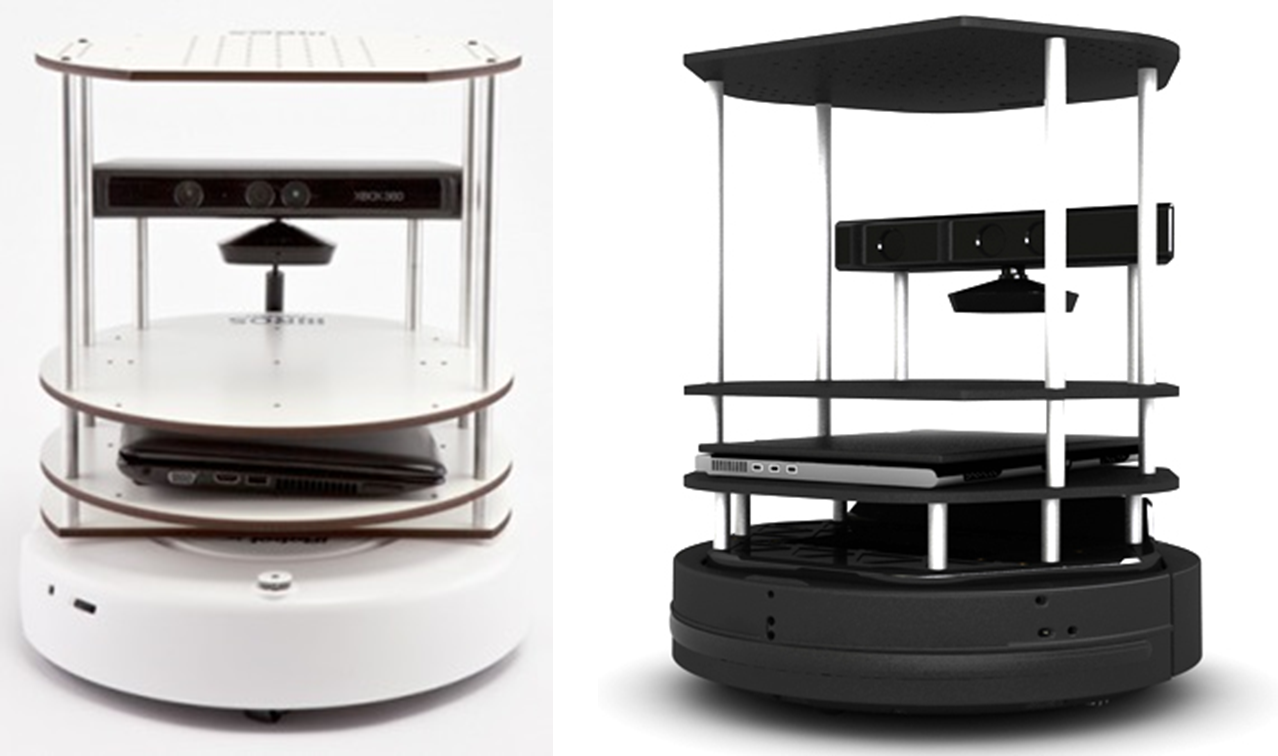
\includegraphics[width=\columnwidth]{pictures/chapter9/pic_09_01.png}
  \caption{タートルボット1(左)とタートルボット2(右)}
\end{figure}

%-------------------------------------------------------------------------------
\subsection{タートルボット2}

タートルボット2は、2012年10月に公開されたロボットプラットフォームである。柱やプレートなどの付属品を利用して、ノートパソコンやKinect、その他のセンサやデバイスを搭載できる。タートルボット2の仕様は以下の通りである。

\subsubsection{ハードウェア}
\begin{itemize}
\item Kobuki本体
\item Microsoft Kinect
\item ノートパソコン(OS: Ubuntu、ROSインストール済み)
\item Kinect 取り付け治具
\item TurtleBot 柱
\item TurtleBot プレート
\end{itemize}

\subsubsection{ソフトウェア}
\begin{itemize}
\item タートルボットSDK
\item visualization、planning、perception、control and error handlingライブラリ
\item デモアプリケーション(https://github.com/turtlebot/turtlebotからダウンロード可能)
\end{itemize}

%-------------------------------------------------------------------------------
\section{移動ロボットKobuki}\index{移動ロボットKobuki}


Kobukiは、Yujin Robot社が開発し、タートルボット2で採用された研究用移動ロボットプラットフォームである。図9-2にKobukiとタートルボット2を示す。移動ロボットプラットフォームとは、移動ロボット開発に必要な基本的な機能を搭載したハードウェアであり、多様なセンサやロボットアームが装備できるなど、様々な拡張が可能である。  Kobukiには、標準でバンパーセンサ、落下検知センサ、ホイールドロップセンサ、高解像度の車輪エンコーダ、モータ、3軸ジャイロセンサ、デジタル入出力端子、アナログ入力端子、バッテリーが搭載されている。  本節では、Kobukiのハードウェア構成について解説する。

\begin{figure}[ht]
  \centering
  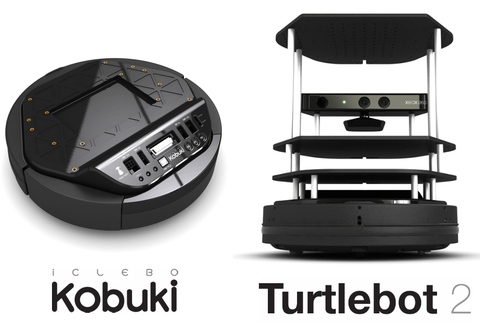
\includegraphics[width=\columnwidth]{pictures/chapter9/pic_09_02.png}
  \caption{Kobukiとタートルボット2}
\end{figure}


%-------------------------------------------------------------------------------
\subsection{Kobukiの構成と仕様}

Kobukiと付属機器を図9-3に示す。基本的な構成は、Kobuki本体、ドッキングステーション、リチウムイオン電池、充電アダプタ、プレートと柱、USBケーブルである。本章では、これに加えて9.4.2項に示すように、プログラム開発用のデスクトップPCとノートパソコンを使用する。

\begin{figure}[ht]
  \centering
  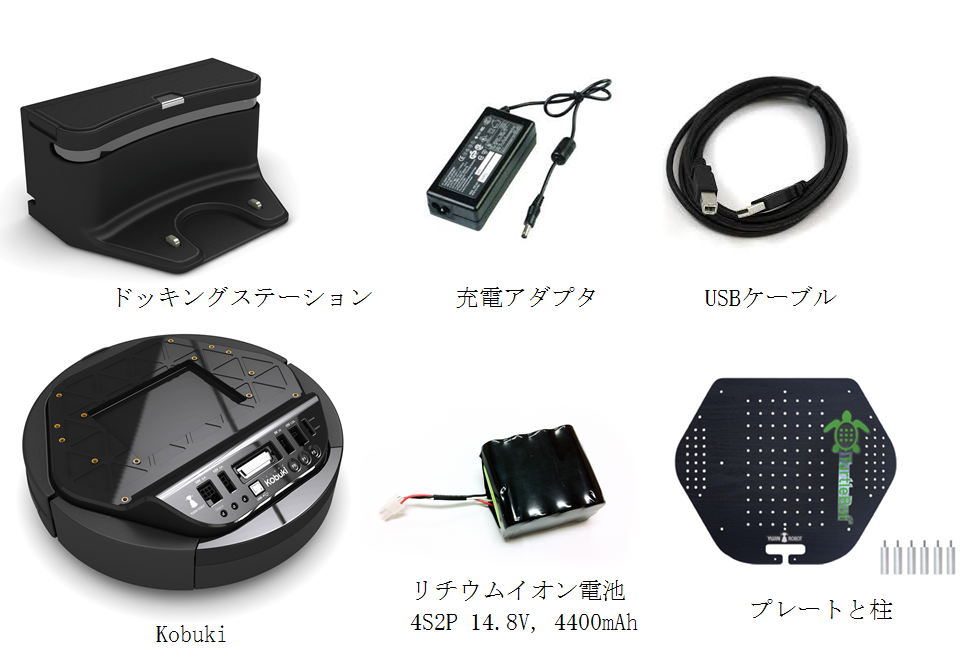
\includegraphics[width=\columnwidth]{pictures/chapter9/pic_09_03.png}
  \caption{Kobuki本体と付属機器}
\end{figure}


図9-4にKobuki本体のモータ、センサ、端子などの位置を示す。Kobukiのより詳しい仕様は、次のURLを参照してほしい。図9-5に示すように、バンパーが装着されている部分がKobukiの前方である。

http://kobuki.yujinrobot.com/home-kr/about/specifications/

\begin{figure}[ht]
  \centering
  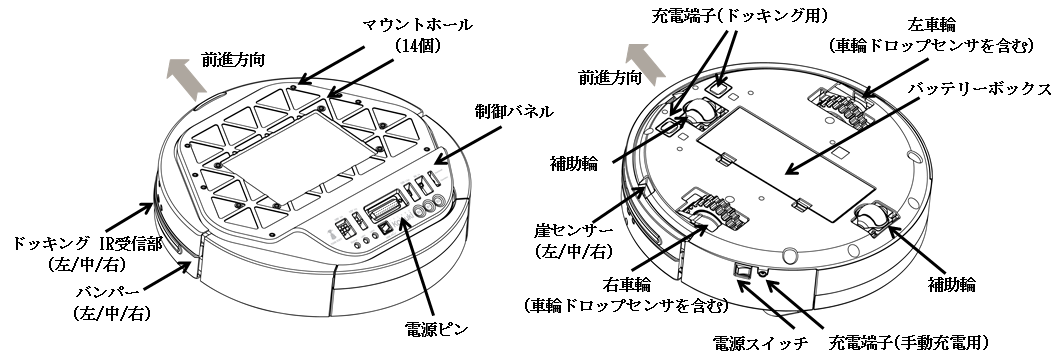
\includegraphics[width=\columnwidth]{pictures/chapter9/pic_09_04.png}
  \caption{Kobuki本体の各部分の説明}
\end{figure}


\begin{figure}[ht]
  \centering
  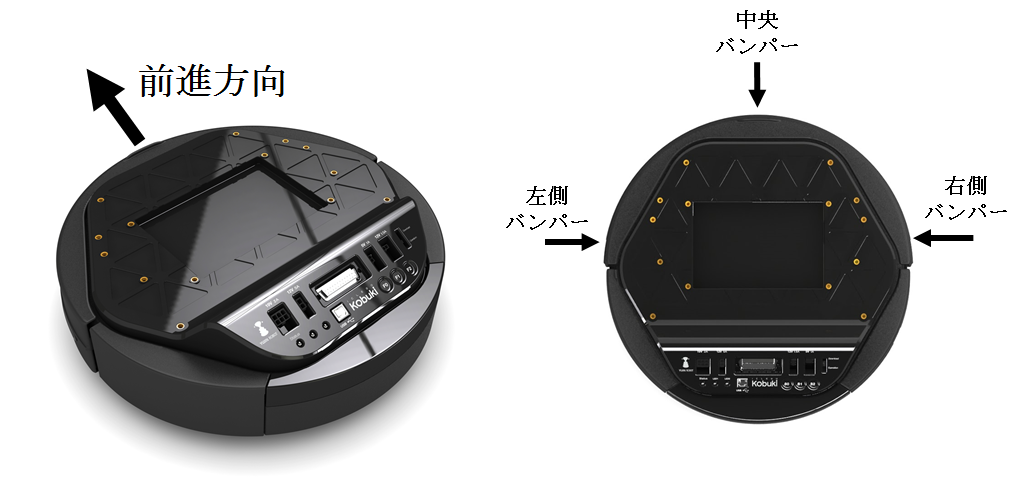
\includegraphics[width=\columnwidth]{pictures/chapter9/pic_09_05.png}
  \caption{Kobukiのバンパーと前進方向}
\end{figure}

\begin{exercise}[KobukiのCAD図面の入手方法]
  Kobukiに新たな機器やセンサを追加する際、正確な寸法が必要になる。Kobukiの寸法を記入したCAD図面は、以下のURLから入手できる。2次元モデルはDWG、PDF形式で、3次元モデルは、IGS、STEP、STL形式で提供されている。
  \begin{itemize}
    \item  2次元モデル:  http://files.yujinrobot.com/kobuki/hardware/drawings/
    \item  3次元モデル:  http://files.yujinrobot.com/kobuki/hardware/models/
  \end{itemize}
\end{exercise}

%-------------------------------------------------------------------------------
\subsection{Kobuki制御パネルと電源オプション}

Kobukiの後部には、図9-6のような制御パネルがある。制御パネルには、搭載するセンサ用の外部電源  、簡単なステータスを表示するLEDやUSB端子、ボタン、スイッチがある。

\begin{figure}[ht]
  \centering
  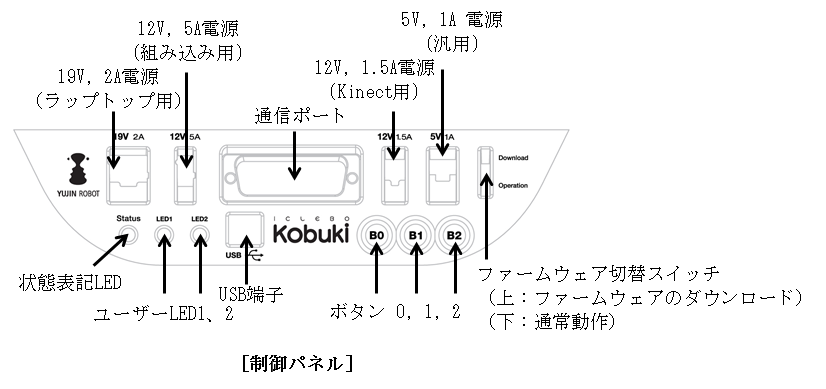
\includegraphics[width=\columnwidth]{pictures/chapter9/pic_09_06.png}
  \caption{Kobukiの制御パネル}
\end{figure}

図9-7のように、Kobukiはノートパソコン、組み込みボード、Kinectなどの外部機器用に4つの電源ピンを備えている。Kobukiの電源を外部機器で利用したいとき、この電源ピンを使用すればよい。電源ピンのコネクタを以下に示す。

\begin{figure}[ht]
  \centering
  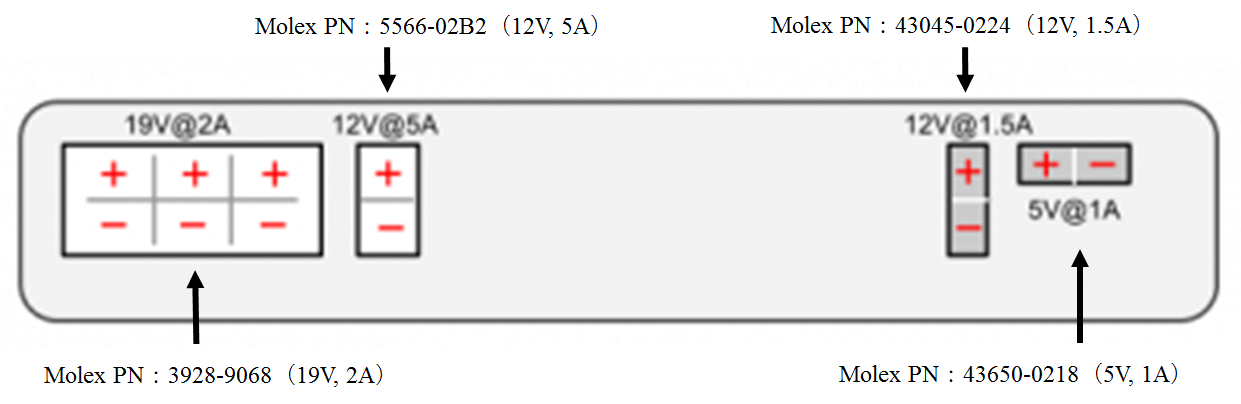
\includegraphics[width=\columnwidth]{pictures/chapter9/pic_09_07.png}
  \caption{Kobuki制御パネル上の電源ピン}
\end{figure}

%-------------------------------------------------------------------------------
\subsection{Kobukiドッキングステーション}

Kobukiの充電は、ユーザーが直接充電アダプタを接続する方法と、ロボットが自ら充電ステーション(ドッキングステーション、図9-8)へ移動して充電  する方法がある。

\begin{figure}[ht]
  \centering
  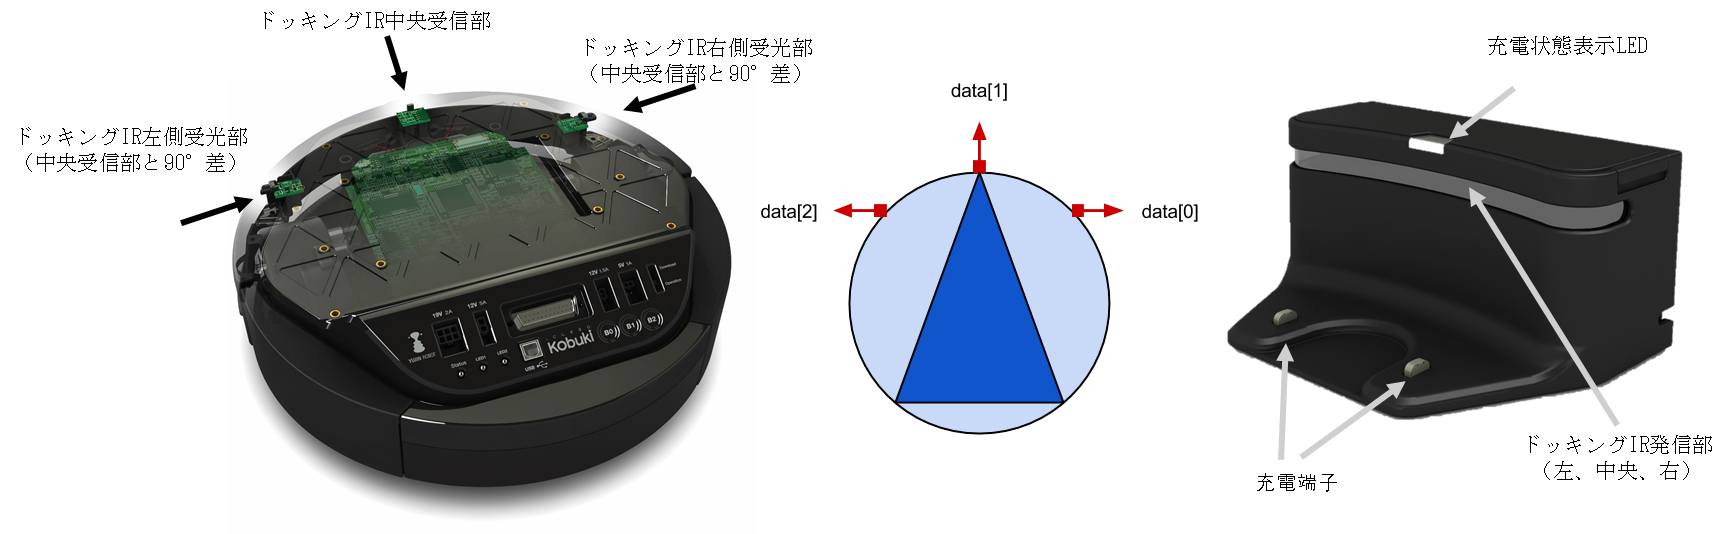
\includegraphics[width=\columnwidth]{pictures/chapter9/pic_09_08.png}
  \caption{Kobukiドッキングステーション}
\end{figure}

%-------------------------------------------------------------------------------
\subsection{Kobuki通信ポート}

Kobukiの制御パネルには、図9-9のような D-Sub コネクタ(25ピン)の通信ポートがある。

\begin{figure}[ht]
  \centering
  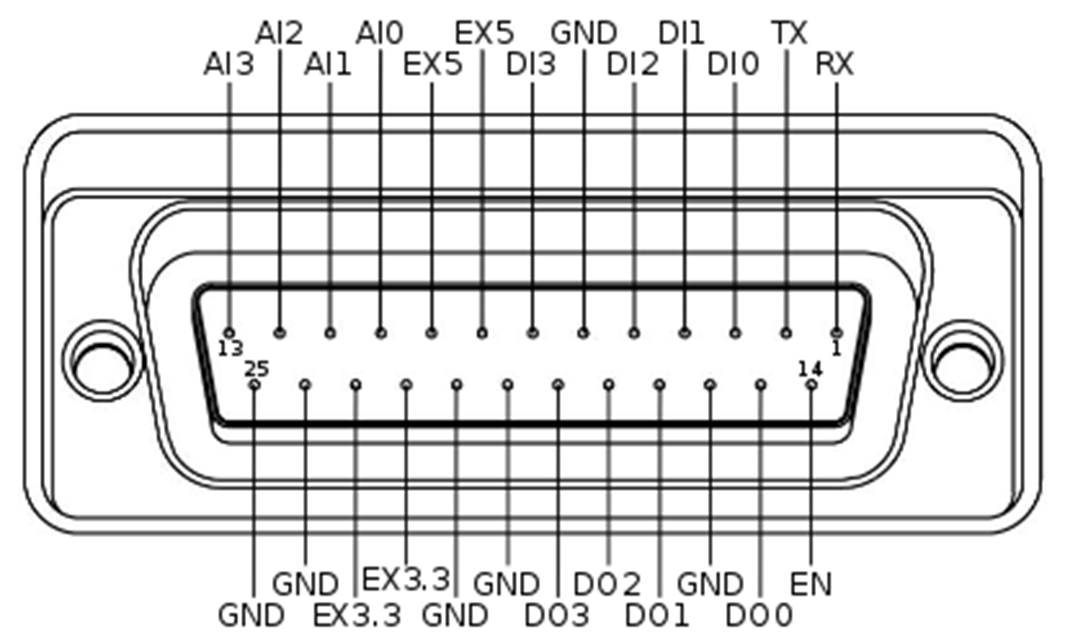
\includegraphics[width=\columnwidth]{pictures/chapter9/pic_09_09.png}
  \caption{KobukiのD-Subコネクタ(25ピン)通信ポート}
\end{figure}

この通信ポートの各ピンの名称、機能を表9-1に示す。

\begin{table}[h]
\centering
\begin{tabular}{l l l l}
\toprule
\textbf{ピン番号} & \textbf{名称} & \textbf{機能} & \textbf{備考}\\
\midrule
1,2 & RX, TX  & シリアル通信  & RS232, 3.3V \\
3,4,5,7 & DI0, DI1, DI2, DI3  & デジタル入力  & High: 3.3 - 5V, Low: 0V \\
8,9 & EX5 & 5V電源  & 1A \\
10,11,12,13 & AI0, AI1, AI2, AI3  & アナログ入力  & 12bit ADC: 0~4095, 0~3.3V \\
14  & EN  & 外部ボード検出 & 外部GND \\
15,17,18,19 & DO0, DO1, DO2, DO3  & デジタル出力  & Open-drain, プルアップ抵抗が必要 \\
22,23 & EX3.3 & 3.3V & 電源 1A \\
6,16,20,21,24,25  & GND & グラウンド & GND \\
\bottomrule
\end{tabular}
\caption{通信ポートの説明}
\end{table}


\subsubsection{SBCやMCUとの接続}
USBケーブルを介してKobukiとノートパソコンを接続すれば、そのパソコンから制御できる。  USBが使用できないパソコンやボードコンピュータ(Single Board Computer(SBC)やMicro Control Unit(MCU))では、通信ポートを利用してシリアル通信で制御することもできる。通信ポートを使用する際の注意点を以下に示す。

\begin{itemize}
\item RS-232インターフェース方式の接続  : Kobukiのシリアルポート(通信ポートの1,2番ピン)の使用電圧は標準3.3V、最大5V   である。これ以外の通信基準電圧を使用する 産業用組込みLinuxボード等を接続する   には、MAX232チップなどのライントランシーバ(line transceiver)を用いる必要がある(図9-10左図)。
\item MCUとの接続: Kobukiのシリアルピン入出力は3.3V〜5Vまで許容されるので、一般的なMCUは図9-10右図のように直接接続することができる  。
\item 通信プロトコルの仕様: 通信プロトコルの仕様は、次のURLに記載されている。http://yujinrobot.github.io/kobuki/doxygen/enAppendixProtocolSpecification.html
\end{itemize}

\begin{figure}[ht]
  \centering
  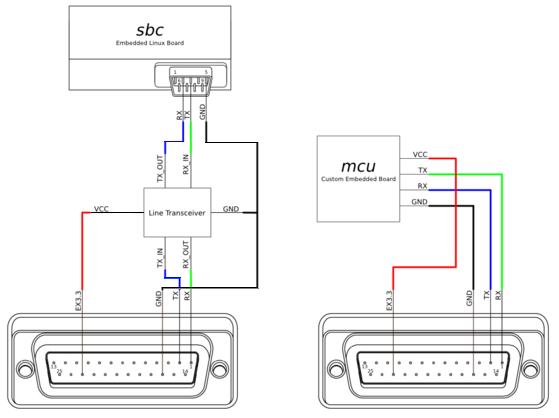
\includegraphics[width=\columnwidth]{pictures/chapter9/pic_09_10.png}
  \caption{SBC、MCUとの接続方法}
\end{figure}

\begin{exercise}[通信ポート関連回路図の入手先]
通信ポートに関連した回路図は以下のURLから入手できる。
http://kobuki.yujinrobot.com/files/5613/5526/9189/io\_port\_121024.pdf
\end{exercise}

%-------------------------------------------------------------------------------
\section{Kobukiソフトウェア}\index{Kobukiソフトウェア}

ROSを利用してKobukiを制御するために、以下の4つのメタパッケージが提供されている  。メタパッケージ(metapackage)とは、同じ目的のパッケージを複数集めたセットである。

\subsubsection{kobukiメタパッケージ}

Kobuki関連のソフトウェアがほぼすべて含まれ、通常使用されるパッケージのほとんどが提供されている。

\begin{itemize}
\item リポジトリ: https://github.com/yujinrobot/kobuki
\item パッケージ: kobuki\_auto\_docking、kobuki\_bumper2pc、kobuki\_capabilities、kobuki\_controller\_tutorial、kobuki\_description、kobuki\_keyop、kobuki\_node、kobuki\_random\_walker、kobuki\_rapps、kobuki\_safety\_controller、kobuki\_testsuite
\end{itemize}

\subsubsection{kobuki\_desktopメタパッケージ}

動力学シミュレータGazeboを用いたシミュレーション用パッケージ   である

\begin{itemize}
\item リポジトリ: https://github.com/yujinrobot/kobuki\_desktop
\item パッケージ: kobuki\_dashboard、kobuki\_gazebo、kobuki\_gazebo\_plugins、kobuki\_qtestsuite


\subsubsection{kobuki\_softメタパッケージ}

可視化ツールであるRVizを利用したシミュレーション用パッケージである。

\begin{itemize}
\item リポジトリ: https://github.com/yujinrobot/kobuki\_soft
\item パッケージ: kobuki\_softapps、kobuki\_softnode
\end{itemize}

\subsubsection{kobuki\_coreメタパッケージ}

Kobukiのハードウェアを直接操作するためのドライバパッケージである。

\begin{itemize}
\item リポジトリ: https://github.com/yujinrobot/kobuki\_core
\item パッケージ: kobuki\_dock\_drive、kobuki\_driver、kobuki\_ftdi
\end{itemize}

以下では、各メタパッケージの詳細について説明する。

\begin{exercise}[Kobuki SDK]
  Kobuki SDKは Kobuki制御用のWindows/Linux向けC/C ++ APIライブラリである。ROSパッケージを使用しない場合は、これらのライブラリを利用できる。
  http://yujinrobot.github.io/kobuki/doxygen/enMainPage.html

  \begin{itemize}
  \item Windows用
  http://files.yujinrobot.com/kobuki/windows/sdk-kobuki-x86-vs10-release.zip
  \item Linux用
  https://github.com/yujinrobot/kobuki\_core.git
  \end{itemize}
\end{exercise}

\begin{exercise}[OpenRTMサポートソフトウェア]
KobukiはROS以外にRTミドルウエアのOpenRTMにも対応している。詳細は、OpenRTM公式ホームページのKobukiコンポーネントで確認できる。
http://openrtm.org/openrtm/node/273
\end{exercise}

%-------------------------------------------------------------------------------
\subsection{kobukiメタパッケージ}

kobukiメタパッケージには、Kobukiに関連するパッケージがほぼすべて含まれている。ここでは、主なパッケージについて説明していく。

\begin{itemize}
\item wiki: http://wiki.ros.org/kobuki
\item リポジトリ: https://github.com/yujinrobot/kobuki
\end{itemize}

\subsubsection{kobuki\_node}

\begin{itemize}
\item wiki: http://wiki.ros.org/kobuki\_node
\item Linux用Kobuki起動ドライバをROS用に再構成したパッケージである。また、nodelet(コラム参照)よりマルチスレッド機能を提供する。
\end{itemize}

\subsubsection{kobuki\_keyop}

\begin{itemize}
\item wiki: http://wiki.ros.org/kobuki\_keyop
\item キーボードでKobukiを遠隔操縦するためのパッケージである。
\end{itemize}

\subsubsection{kobuki\_random\_walker}

\begin{itemize}
\item wiki: http://wiki.ros.org/kobuki\_random\_walker
\item Kobukiに搭載した、バンパー、落下検知、ホイールドロップなどのセンサを用いて、周囲の環境をランダム走行するためのパッケージである。通常、Kobukiの基本動作を確認する際に使われる。
\end{itemize}

\subsubsection{kobuki\_safety\_controller}

\begin{itemize}
\item wiki: http://wiki.ros.org/kobuki\_safety\_controller
\item 搭載したセンサ情報に基づき、Kobukiを安全に制御するためのパッケージである。例えば、前進すれば落下すると予想されたときには、ユーザーが前進コマンドを与えても、それを無視してKobukiを停止する、などの制御が可能である。
\end{itemize}

\subsubsection{kobuki\_controller\_tutorial}

\begin{itemize}
\item wiki:  http://wiki.ros.org/kobuki\_controller\_tutorial
\item Kobukiの制御法を学ぶためのチュートリアルパッケージである。例えば、Kobukiのバンパーが押されたときにLEDを点滅する機能などが解説されている。
\end{itemize}

\subsubsection{kobuki\_description}

\begin{itemize}
\item wiki: http://wiki.ros.org/kobuki\_description)
\item Kobukiのシミュレーションと可視化のための3次元モデル(URDFモデル)が含まれる。
\end{itemize}

\subsubsection{kobuki\_auto\_docking}

\begin{itemize}
\item wiki: http://wiki.ros.org/kobuki\_auto\_docking
\item Kobukiが自律的にドッキングステーションに接続  して、充電する動作に対するパッケージである。
\end{itemize}

\begin{exercise}[nodeletとは?]
nodeletは同じコンピュータ、同じプロセスで複数のプログラムを起動する方法であり、ROSのパッケージとして提供される。これを使えば、ROS上で複数のプログラム(スレッド)が同時に実行できる。
\end{exercise}

%-------------------------------------------------------------------------------
\subsection{kobuki\_desktopメタパッケージ}

kobuki\_desktopメタパッケージには、Kobukiを用いたシミュレーションと可視化に関連するパッケージがすべて含まれている。主要なパッケージを以下に示す。

\begin{itemize}
\item wiki: http://wiki.ros.org/kobuki\_desktop
\item リポジトリ: https://github.com/yujinrobot/kobuki\_desktop
\end{itemize}

\subsubsection{kobuki\_dashboard}

\begin{itemize}
 \item wiki:  http://wiki.ros.org/kobuki\_dashboard
\item rqtによるKobukiの状態の可視化のためプラグインである。ロボットおよびノートパソコンのバッテリー情報、エラー、警告情報をGUIプログラムで確認できる。
\end{itemize}

\subsubsection{kobuki\_gazebo}

\begin{itemize}
\item wiki: http://wiki.ros.org/kobuki\_gazebo
\item 3次元シミュレーション環境GazeboでKobukiを使用するために必要となる。
\end{itemize}

\subsubsection{kobuki\_gazebo\_plugins}

\begin{itemize}
\item wiki: http://wiki.ros.org/kobuki\_gazebo\_plugins
\item kobuki\_gazeboとともに使用するパッケージで、バンパー、落下検知、オドメトリ(走行距離に基づく位置情報)、IMU等のセンサを利用し、Kobukiを仮想的に制御できる。
\end{itemize}

%-------------------------------------------------------------------------------
\subsection{kobuki\_softメタパッケージ}

kobuki\_softメタパッケージでは、可視化ツールRVizでKobukiの動作をシミュレーションする環境を提供する。

\begin{itemize}
\item wiki: http://wiki.ros.org/kobuki\_soft
\item リポジトリ: https://github.com/yujinrobot/kobuki\_soft
\end{itemize}

\subsubsection{kobuki\_softnode}

\begin{itemize}
\item wiki: http://wiki.ros.org/kobuki\_softnode
\item Kobukiの動作をシミュレーションするパッケージである。RVizで実行することができる。
\end{itemize}

\subsubsection{kobuki\_softapps}

\begin{itemize}
\item wiki: http://wiki.ros.org/kobuki\_softapps
\item kobuki\_softnodeの関連パッケージで、ナビゲーションなどのアプリケーションが含まれる。
\end{itemize}

%-------------------------------------------------------------------------------
\subsection{kobuki\_coreメタパッケージ}

Kobukiやドッキングステーションを直接操作するためのドライバパッケージである。

\begin{itemize}
\item wiki: http://wiki.ros.org/kobuki\_core
\item リポジトリ: https://github.com/yujinrobot/kobuki\_core
\end{itemize}

\subsubsection{kobuki\_dock\_drive}

\begin{itemize}
\item wiki: http://wiki.ros.org/kobuki\_dock\_drive
\item ドッキングステーションを利用するためのパッケージが含まれる。
\end{itemize}

\subsubsection{kobuki\_driver}

\begin{itemize}
\item wiki: http://wiki.ros.org/kobuki\_driver
\item C++でKobukiを制御するためのドライバパッケージである。ROSを使わずにKobukiを制御できる  。
\end{itemize}

%-------------------------------------------------------------------------------
\section{Kobukiを用いたROSアプリケーション開発}\index{Kobukiを用いたROSアプリケーション開発}

前節では、KobukiのハードウェアとKobukiを用いたROSアプリケーション開発  のためのパッケージを紹介した。本節では、Kobukiを実際に動かしながら、前節で紹介したパッケージの動作を確認する。

%-------------------------------------------------------------------------------
\subsection{Kobukiの動作確認}

Kobukiには、単独でも動作する簡単なテストプログラムがインストールされている。まずはテストプログラムを実行して、Kobukiの動作を確認する  。

\begin{enumerate}
\item Kobukiを床の安全な場所に置く。机の上のようにKobukiが落下する可能性がある場所は避ける。
\item Kobukiの電源スイッチをオンにする。
\item 電源投入後、3秒以内にKobukiの制御パネルの<B0>ボタンを2秒間押して離す。
\item Kobukiがランダムに動きまわる。動作中、障害物がバンパーにぶつかると、その場回転して再度進む。動作しない場合には、バッテリー切れや故障の可能性がある。
\end{enumerate}

%-------------------------------------------------------------------------------
\subsection{開発環境}

本章で用いる開発環境を図9-11に示す。開発環境は、必ずしも本書のとおりである必要はない。

\subsubsection{デスクトップPC}

Kobukiの操縦、センサ処理、ナビゲーションを担当する。すべての開発をこのコンピュータで行うとともに、ROSのマスター   として用いる。

\begin{itemize}
\item Ubuntu 14.04 LTS 64bit(Trusty Tahr)
\item ROS Indigo
\item ROSパッケージ: Kobuki関連のすべてのパッケージ
\end{itemize}

\subsubsection{ノートパソコン(ラップトップPC)}

Kobukiに搭載するPCであり、Kobukiと直接通信して動作コマンドを送り、またセンサデータをデスクトップPCに送信する。
\begin{itemize}
\item Ubuntu 14.04 LTS 64bit(Trusty Tahr)
\item ROS Indigo
\item ROSパッケージ: ros-indigo-kobukiとros-indigo-kobuki-core
\end{itemize}

\begin{figure}[ht]
  \centering
  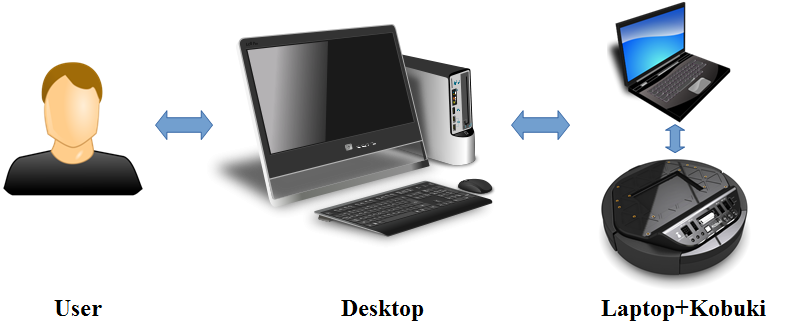
\includegraphics[width=\columnwidth]{pictures/chapter9/pic_09_11.png}
  \caption{開発環境}
\end{figure}

%-------------------------------------------------------------------------------
\subsection{Kobukiパッケージのインストール}

開発環境が整ったら、デスクトップPCとノートパソコンにKobuki関連パッケージをインストールする。

\subsubsection{ノートパソコンへのインストール}

\setcounter{num}{0}

\stepcounter{num}\circled{\thenum} ROS Indigoのインストール

Kobukiに搭載したノートパソコンにROS Indigoバージョンをインストールする。手順は2.1節を参照してほしい。

\stepcounter{num}\circled{\thenum} ノートパソコンのROSの環境設定

「.bashrc」ファイルに記述されたROS\_MASTER\_URIにはデスクトップPCのIPアドレスを設定し、ROS\_HOSTNAMEにはノートパソコンのIPアドレスを設定する。それぞれのIPアドレスは、ターミナルウィンドウを開いてifconfigコマンドを入力すれば確認できる。「.bashrc」ファイルの変更方法の詳細については、2.2節を参考にしてほしい。

\begin{lstlisting}[language=bash]
export ROS_HOSTNAME = %*ノートパソコンのIPアドレス*)
export ROS_MASTER_URI = http: //%*デスクトップPCのIPアドレス*):11311
\end{lstlisting}

\stepcounter{num}\circled{\thenum} Kobukiの制御に必要なパッケージのインストール

Kobukiを制御するために必要なパッケージros-indigo-kobukiとros-indigo-kobuki-coreをインストールする。

\begin{lstlisting}[language=ROS]
$ sudo apt-get install ros-indigo-kobuki ros-indigo-kobuki-core
\end{lstlisting}

\stepcounter{num}\circled{\thenum} SSHのインストール

以降では、通信ソフトウェアであるSSH(Secure Shell)  を利用してデスクトップPCから接続するため、SSHをインストールする。

\begin{lstlisting}[language=ROS]
$ sudo apt-get install ssh
\end{lstlisting}


\subsubsection{デスクトップPCへのインストール}

\setcounter{num}{0}

\stepcounter{num}\circled{\thenum} ROS Indigoのインストール

デスクトップPCにも、ノートパソコンと同様にROS Indigoをインストールする。

\stepcounter{num}\circled{\thenum} デスクトップPCのROSの環境設定

ROS\_MASTER\_URIとROS\_HOSTNAMEにデスクトップPCのIPアドレスを設定する。

\begin{lstlisting}[language=bash]
export ROS_HOSTNAME = %*デスクトップPCのIPアドレス*)
export ROS_MASTER_URI = http: //%*デスクトップPCのIPアドレス*):11311
%*あるいは*)
export ROS_MASTER_URI = http: //${ROS_HOSTNAME}:11311
\end{lstlisting}

\stepcounter{num}\circled{\thenum} Kobuki関連のすべてのパッケージのインストール
次のように、Kobukiの制御に関連するすべてのパッケージをインストールする。ただし、シミュレーションに関連したパッケージのインストールについては、9.10節で解説する。

\begin{lstlisting}[language=ROS]
$ sudo apt-get install ros-indigo-kobuki*
\end{lstlisting}

以上で、基本的な開発環境が構築できた。次節では実際に簡単なプログラムを実行する。

\begin{exercise}[小型SBC(Single Board Computer)の使用]
タートルボットの制御には、ノートパソコンではなくラズベリーパイなどの小型SBCを用いることもできる。ただし、Kinect、Xtionなどデプスカメラを使用する場合には、高性能なボードが必要となる。
\end{exercise}

%-------------------------------------------------------------------------------
\section{Kobukiのリモートコントロール}\index{Kobukiのリモートコントロール}

\setcounter{num}{0}

ROSを利用してデスクトップPCからノートパソコンに動作指令を送り、Kobukiを操縦してみよう。

\stepcounter{num}\circled{\thenum} マスターの起動
デスクトップPCで、ターミナルウィンドウを開いてroscoreを実行する。なお、以降で説明する各コマンドはすべて、新しいターミナルウィンドウを開いて実行する必要がある。

\begin{lstlisting}[language=ROS]
$ roscore
\end{lstlisting}

\stepcounter{num}\circled{\thenum} SSHによるデスクトップPCからノートパソコンへの接続
KobukiとノートパソコンをUSBケーブルで接続し、電源スイッチをオンにする。次に、デスクトップPCからSSHでノートパソコンに接続する。  ターミナルウィンドウで「ssh ユーザー名@ノートパソコンのIPアドレス」のように入力すると、ノートパソコンに接続できる。

\begin{lstlisting}[language=bash]
$ %*sshユーザー名*)@%*ノートパソコンのIPアドレス*)
\end{lstlisting}

\stepcounter{num}\circled{\thenum} Kobukiポートの作成

ノートパソコンに接続したターミナルウィンドウで、次のようにcreate\_udev\_rulesノードを実行する。これにより、「/dev/kobuki」ポートが生成される。

\begin{lstlisting}[language=ROS]
$ rosrun kobuki_ftdi create_udev_rules
\end{lstlisting}


上記を実行した後、いちどUSBケーブルを抜いて、再度接続する。「ls -l  /dev/kobuki」コマンドで接続ポートを確認できる。

\begin{lstlisting}[language=ROS]
$ ls -l /dev/kobuki
lrwxrwxrwx 1 root root 7 Aug 24 14:26 /dev/kobuki -> ttyUSB0
\end{lstlisting}


上の例では、「/dev/kobuki」のポートはttyUSB0に接続されている。ttyUSB0,1,2など接続状態が変わっても   、create\_udev\_rulesノードを実行すれば「/dev/kobuki」という統一されたポートを使用できる。

\stepcounter{num}\circled{\thenum} Kobukiの起動
ノートパソコンに接続したターミナルウィンドウで次のコマンドを実行すると、ビープ音が鳴り、初期設定の完了後に待機状態となる。

\begin{lstlisting}[language=ROS]
$ roslaunch kobuki_node minimal.launch --screen
\end{lstlisting}

ノートパソコン上で実行する必要があるノードは以上である。このノードを終了  するには、<Ctrl> + <c>を押す。

\stepcounter{num}\circled{\thenum} キーボード制御ノードの起動
デスクトップPC上で新しいターミナルウィンドウを開き、次のように入力する。

\begin{lstlisting}[language=ROS]
$ roslaunch kobuki_keyop keyop.launch
\end{lstlisting}

この際、\stepcounter{4}\circled{\thenum}で使用したターミナルウィンドウはそのままにしておく。\stepcounter{5}\circled{\thenum}を実行したターミナルウィンドウでキーボードを押すと、Kobukiを遠隔制御できる。Kobukiの操作に使用するキーの一覧を以下に示す。


\begin{itemize}
\item 方向キー↑: 指定された並進速度で前進する。(一回押すごとに0.5 m/secずつ速度が増加)
\item 方向キー↓: 指定された並進速度で後進する。(一回押すごとに0.5 m/secずつ速度が増加)
\item 方向キー←: 指定された回転速度で反時計回りに回転する。(一回押すごとに0.33 rad/secずつ速度が増加)
\item 方向キー→: 指定された回転速度で時計方向に回転する。(一回押すごとに0.33 rad/secずつ速度が増加)
\item スペースバー: 並進速度と回転速度を初期化する。
\item d: モータを無効にする。(Kobukiが動作不能状態になる)
\item e: モータを有効にする。(Kobukiが動作可能状態になる)
\item q: 終了
\end{itemize}

\begin{exercise}[kobukiの安全な操作方法(セーフモード)]
セーフモードとは、ユーザーの不注意でKobukiが損傷するのを防止するため、急激な速度変化を防ぎ、またバンパー、落下検知センサ、ホイールドロップセンサの値から危険な状況を回避するモードである。  次の命令で実行する。

\begin{lstlisting}[language=ROS]
$ roslaunch kobuki_keyop safe_keyop.launch
\end{lstlisting}

\end{exercise}

ここまで、基本的な開発環境を構築し、Kobukiの動作を確認した。次節では、これまでに紹介したKobuki関連パッケージのノードを実際に使用した場合の動作を説明する。

%-------------------------------------------------------------------------------
\section{Kobukiのトピック}\index{Kobukiのトピック}

本節では、実際にKobukiを動作させ、配信、購読されているトピックを確認するとともに、それぞれのトピックを使ったKobukiの制御について解説する。

%-------------------------------------------------------------------------------
\subsection{kobuki\_nodeパッケージ  で使用されるトピック}

ノートパソコンに接続したターミナルウィンドウで、「roslaunch kobuki\_node minimal.launch 」コマンドを実行してKobukiを起動する。kobuki\_nodeパッケージのmobile\_baseノードが動作している間 、Kobukiのバンパー、落下検知センサ、ホイールドロップセンサ、モータ駆動部などの情報はトピックメッセージとして配信されているので、これを確認してみる。
デスクトップPCでroscoreのみを実行し、それ以外のノードを実行していない状態で、「rostopic list」コマンドでトピックのリストを見てみると、「/rosout」、「/rosout\_agg」しか現れない。しかし、ノートパソコンに接続したターミナルウィンドウでkobuki\_nodeパッケージのminimal.launchを実行すると、次のようにkobuki\_nodeパッケージで使用されるさまざまなトピックを確認できる。

\begin{lstlisting}[language=ROS]
$ rostopic list
/diagnostics
/diagnostics_agg
/diagnostics_toplevel_state
/joint_states
/mobile_base/commands/controller_info
/mobile_base/commands/digital_output
/mobile_base/commands/external_power
/mobile_base/commands/led1
/mobile_base/commands/led2
/mobile_base/commands/motor_power
/mobile_base/commands/reset_odometry
/mobile_base/commands/sound
/mobile_base/commands/velocity
/mobile_base/controller_info
/mobile_base/debug/raw_control_command
/mobile_base/debug/raw_data_command
/mobile_base/debug/raw_data_stream
/mobile_base/events/bumper
/mobile_base/events/button
/mobile_base/events/cliff
/mobile_base/events/digital_input
/mobile_base/events/power_system
/mobile_base/events/robot_state
/mobile_base/events/wheel_drop
/mobile_base/sensors/core
/mobile_base/sensors/dock_ir
/mobile_base/sensors/imu_data
/mobile_base/sensors/imu_data_raw
/mobile_base/version_info
/mobile_base_nodelet_manager/bond
/odom
/rosout
/rosout_agg
/tf
...
\end{lstlisting}

GUI環境で確認するには、「rqt\_graph」コマンドを使用する。これにより、実行されたすべてのノードとトピックが確認できる。

%-------------------------------------------------------------------------------
\subsection{購読者トピック}

前節で確認したトピック  は、Kobukiのノートパソコンが受信している購読者トピックと、ノートパソコンから送信される配信者トピックに分けることができる。このうち、購読者トピックは次の通りである。

\begin{lstlisting}[language=ROS]
/mobile_base/commands/controller_info
/mobile_base/commands/digital_output
/mobile_base/commands/external_power
/mobile_base/commands/led1
/mobile_base/commands/led2
/mobile_base/commands/motor_power
/mobile_base/commands/reset_odometry
/mobile_base/commands/sound
/mobile_base/commands/velocity
\end{lstlisting}

それぞれのトピックについて、より詳しい説明を表9-2に示す1 。例えば、「velocity」はKobukiの動作速度を設定するトピックである。ユーザーは、ロボットの前進、後進、左右旋回、静止などを、このトピックを介して制御できる。

\begin{table}[h]
\centering
\begin{tabular}{l l l}
\toprule
\textbf{名} & \textbf{タイプ} & \textbf{機能}\\
\midrule
controller\_info & kobuki\_msgs/ControllerInfo  & PIDゲイン設定(デフォルトのPID ゲイン: Kp = 100、Ki = 0.1、Kd = 2)\\
digital\_output  & kobuki\_msgs/DigitalOutput & デジタル出力ピン制御 \\
external\_power  & kobuki\_msgs/ExternalPower & 外部電源On/Off \\
led1 & kobuki\_msgs/Led & LED1制御 \\
led2  & kobuki\_msgs/Led & LED2制御 \\
motor\_power & kobuki\_msgs/MotorPower  & KobukiモータOn/Off \\
reset\_odometry  & std\_msgs/Empty  & オドメトリ(走行距離に基づく位置情報)のリセット \\
sound & kobuki\_msgs/Sound & ビープ音 \\
velocity  & geometry\_msgs/Twist & 前進後進速度(m/s)、回転速度(rad/s)の設定 \\
\bottomrule
\end{tabular}
\caption{Kobukiの購読者トピック}
\end{table}

%-------------------------------------------------------------------------------
\subsection{購読者トピックによるKobukiの制御}

前項で示した購読者トピックを利用して、ユーザーはKobukiを様々に制御できる。  ここでは、このうち代表的な購読者トピックの使い方を紹介する  。

\subsubsection{led1トピック}

Kobukiの制御パネルのLED1を制御する。新しいターミナルウィンドウを開いて、次のコマンドを入力すると、LED1が点灯する。

\begin{lstlisting}[language=ROS]
$ rostopic pub /mobile_base/commands/led1 kobuki_msgs/Led "value: 1"
\end{lstlisting}

ここで、"value: 1"はvalueオプションが1であることを示す。valueオプションは0〜3まで設定できる  。 0はLEDをオフ、1は緑、2はオレンジ、3は赤で点灯する。

\subsubsection{soundトピック}

Kobukiのビープ音を鳴らすもので、valueオプションで次の0〜6まで設定できる。0: 電源On音、2: 充電開始音、3: ボタンのクリック音、4: エラー発生音、5: 清掃開始音、6: クリーニング終了音である。

\begin{lstlisting}[language=ROS]
$ rostopic pub /mobile_base/commands/sound kobuki_msgs/Sound "value: 6"
\end{lstlisting}

\subsubsection{velocityトピック}

Kobukiの並進速度、回転速度を制御する。ここでKobukiの運動を表現するためにx、y、zの3つの軸を導入する。x軸が前進方向、y軸が右方向、z軸が上方向である。また並進速度の単位はm/s、回転速度はrad/sである。
次の例のようにlinearのxの値に0.2を与えた場合、Kobukiは0.2m/sの速度で前進する。

\begin{lstlisting}[language=ROS]
$ rostopic pub /mobile_base/commands/velocity geometry_msgs/Twist "linear:
x: 0.2
y: 0.0
z: 0.0
angular:
x: 0.0
y: 0.0
z: 0.0"
\end{lstlisting}

また、次の例のようにangularのzの値に1.0を与えた    とき、Kobukiはz軸を中心に反時計回り  に1.0rad/sの速度で回転する。

\begin{lstlisting}[language=ROS]
$ rostopic pub /mobile_base/commands/velocity geometry_msgs/Twist "linear:
x: 0.0
y: 0.0
z: 0.0
angular:
x: 0.0
y: 0.0
z: 1.0"
\end{lstlisting}

%-------------------------------------------------------------------------------
\subsection{配信者トピック}

Kobukiが配信するトピックは、状態の診断関連トピック(diagnostics)、デバッグ関連トピック(debug)、イベント  (状態変化)関連トピック(events)、センサ関連トピック(sensors)、ジョイント関連トピック(joint\_states)、制御情報に関連するトピック(controller\_info)、オドメトリ(odom)と座標変換(tf)関連トピックなどがある。

\begin{lstlisting}[language=ROS]
/diagnostics
/diagnostics_agg
/diagnostics_toplevel_state
/joint_states
/mobile_base/controller_info
/mobile_base/debug/raw_control_command
/mobile_base/debug/raw_data_command
/mobile_base/debug/raw_data_stream
/mobile_base/events/bumper
/mobile_base/events/button
/mobile_base/events/cliff
/mobile_base/events/digital_input
/mobile_base/events/power_system
/mobile_base/events/robot_state
/mobile_base/events/wheel_drop
/mobile_base/sensors/core
/mobile_base/sensors/dock_ir
/mobile_base/sensors/imu_data
/mobile_base/sensors/imu_data_raw
/mobile_base/version_info
/mobile_base_nodelet_manager/bond
/odom
/tf
\end{lstlisting}

いくつかの代表的な配信者トピックについて、より詳しい説明を表9-3から表9-6に示す。特に、odom、tf、joint\_states、sensorsの各トピック  は、今後Kobukiを使用する際に特に重要なトピックなので、どのような情報を含んでいるか、理解してほしい。

\begin{table}[h]
\centering
\begin{tabular}{l l l}
\toprule
\textbf{名} & \textbf{タイプ} & \textbf{機能}\\
\midrule
bumper & kobuki\_msgs/BumperEvent & バンパーOn/Offイベント、左(0)、中央(1)、右側(2)のバンパーの状態を示し、通常の状態が0、押した場合は、1である。 \\
button & kobuki\_msgs/ButtonEvent & ボタンOn/Offイベント、ボタン0、1、2の値で、通常の状態が0、押した場合は、1である。\\
cliff & kobuki\_msgs/CliffEvent  & 落下検知イベント、左(0)、中央(1)、右側(2)の崖の検出状態を示し、通常の状態が0、崖と判断される場合、1である。 \\
digital\_input & kobuki\_msgs/DigitalInputEvent & デジタル入力値(DI0、1、2、3) \\
power\_system & kobuki\_msgs/PowerSystemEvent  & 電源の状態を示す。
& & 0 = UNPLUGGED
& & 1 = PLUGGED\_TO\_ADAPTER
& & 2 = PLUGGED\_TO\_DOCKBASE
& & 3 = CHARGE\_COMPLETED
& & 4 = BATTERY\_LOW
& & 5 = BATTERY\_CRITICAL \\
robot\_state & kobuki\_msgs/RobotStateEvent & ロボットのオン/オフライン状態を示す。\\
wheel\_drop  & kobuki\_msgs/WheelDropEvent  & 左(0)、右側(1)車輪がドロップされているかを表し、通常の状態が0、車輪がドロップされている場合が1である。\\
\bottomrule
\end{tabular}
\caption{Kobukiイベント関連トピック}
\end{table}


\begin{table}[h]
\centering
\begin{tabular}{l l l}
\toprule
\textbf{名} & \textbf{タイプ} & \textbf{機能}\\
\midrule
core  & kobuki\_msgs/SensorState  & 50Hz周期制御ですべてのセンサの値を配信するトピックである。 \\
dock\_ir  & kobuki\_msgs/DockInfraRed  & ドッキング充電ステージで走査する赤外線LEDをKobukiが受信したときの、近接値を配信する。
& & NONE = 0
& & NEAR\_LEFT = 1
& & NEAR\_CENTER = 2
& & NEAR\_RIGHT = 4
& & FAR\_LEFT = 16
& & FAR\_CENTER = 8
& & FAR\_RIGHT = 32 \\
imu\_data  & sensor\_msgs/Imu  & ジャイロセンサのデータで、方向とz軸の角速度情報を示す。\\
imu\_data\_raw & sensor\_msgs/Imu  & ジャイロセンサの補正前データでx、y、z軸の各角速度データを示す。これを補正した情報が、前述のimu\_dataトピックである。\\
\bottomrule
\end{tabular}
\caption{Kobukiセンサ関連トピック}
\end{table}

\begin{table}[h]
\centering
\begin{tabular}{l l l}
\toprule
\textbf{名} & \textbf{タイプ} & \textbf{機能}\\
\midrule
raw\_control\_command & std\_msgs/Int16MultiArray & 速度コマンドの送受信値の確認 \\
raw\_data\_command  & std\_msgs/String & ロボットに送信した加工前のバイトストリーム値を確認 \\
raw\_data\_stream & std\_msgs/String & ロボットから受信された加工前のバイトストリーム値を確認 \\
\bottomrule
\end{tabular}
\caption{Kobukiデバッグ関連トピック}
\end{table}

\begin{table}[h]
\centering
\begin{tabular}{l l l}
\toprule
\textbf{名} & \textbf{タイプ} & \textbf{機能}\\
\midrule
odom & nav\_msgs/Odometry & ジャイロとエンコーダ情報に基づいてKobukiのオドメトリ情報を得ることができる。\\
tf & tf2\_msgs/TFMessage & base\_footprintとodom位置の変換値を有する。\\
joint\_states & sensor\_msgs/JointState & 左/右車輪をジョイントとした時の位置、速度、力などを確認可能である。各ユニットは、位置: m、速度: m/s、力: N•mである。\\
diagnostics & diagnostic\_msgs/DiagnosticArray & 1Hz周期で自己診断情報を得ることができる。\\
version\_info & kobuki\_msgs/VersionInfo & Kobukiのハードウェア、ファームウェア、ソフトウェアのなどの情報を得ることができる。\\
\bottomrule
\end{tabular}
\caption{その他の配信者トピック}
\end{table}

%-------------------------------------------------------------------------------
\subsection{配信者トピックによるロボットの状態の把握}

前項で紹介した配信者トピックでは、ロボットのセンサ値、モータの状態、位置などが配信される。  この項では、実際にいくつかのトピックを受信して、現在のロボットの状態を確認してみよう。

\subsubsection{bumperトピック}

「/events/bumper」トピックは、3つのバンパー(左  、中央、右)(図9-5参照)の状態を示すことができる。例えば、つぎのように表示される。

\begin{lstlisting}[language=ROS]
$ rostopic echo /mobile_base/events/bumper
----
bumper: 1 %*(中央のバンパーが押されている)*)
state: 1
----
bumper: 1 %*(中央のバンパーが押されていない)*)
state: 0
----
\end{lstlisting}

bumperの値は0, 1, 2の3通りで、それぞれ左、中央、右のバンパーを指す。また、stateの値がバンパーの状態を表し、0は押されていない状態、1は押されている状態に対応する。

\subsubsection{coreトピック}

「/sensors/core」トピックでは、bumper、wheel\_drop、cliff、left\_encoder、right\_encoder、left\_pwm、right\_pwm、buttons、charger、battery、bottom、current、over\_current、digital\_input、analog\_inputのセンサの値を配信している。各データの単位は、「kobuki\_msgs/SensorState」注3で確認してほしい。

\begin{lstlisting}[language=ROS]
$ rostopic echo /mobile_base/sensors/core
---
header:
 seq: 357
 stamp:
  secs: 1408945474
  nsecs: 493550939
 frame_id: ''
time_stamp: 64516
bumper: 0
wheel_drop: 0
cliff: 0
left_encoder: 21939
right_encoder: 15968
left_pwm: 0
right_pwm: 0
buttons: 0
charger: 0
battery: 159
bottom: [1539, 1863, 1666]
current: [0, 0]
over_current: 0
digital_input: 0
analog_input: [4067, 4072, 4069, 4069]
---
\end{lstlisting}

\subsubsection{odomトピック}

odomトピックを使用すると、ジャイロとエンコーダに基づいたオドメトリ情報(走行距離に基づく位置情報)を得られる。これは、ナビゲーションに必須の情報である。

\begin{lstlisting}[language=ROS]
$ rostopic echo /odom
---
header:
 seq: 977578
 stamp:
  secs: 1408946075
  nsecs: 676067096
 frame_id: odom
child_frame_id: base_footprint
pose:
 pose:
  position:
   x: 0.413290941207
   y: .0.229207993856
   z: 0.0
  orientation:
   x: 0.0
   y: 0.0
   z: .0.921795503319
   w: 0.387676476022
 covariance: [0.1, 0.0, 0.0, 0.0, 0.0, 0.0, 0.0, 0.1, 0.0, 0.0, 0.0, 0.0, 0.0, 0.0,
1.7976931348623157e+308, 0.0, 0.0, 0.0, 0.0, 0.0, 0.0, 1.7976931348623157e+308, 0.0, 0.0, 0.0,0.0, 0.0, 0.0, 1.7976931348623157e+308, 0.0, 0.0, 0.0, 0.0, 0.0, 0.0, 0.05]
%*~省略~*)
\end{lstlisting}

\subsubsection{tfトピック}

tfトピックは、XY平面上のロボットの中心位置情報であるbase\_footprintと、オドメトリ情報であるodomとの座標変換情報を有する。初期状態ではこの2つの位置情報のみを含むが、KinectやLRFなどを装着した場合に、その取り付け位置を追加で記述することもできる。

\begin{lstlisting}[language=ROS]
$ rostopic echo /tf
---
transforms:
 -
  header:
   seq: 0
   stamp:
    secs: 1408946313
    nsecs: 528813156
   frame_id: odom
  child_frame_id: base_footprint
  transform:
   translation:
    x: 0.413290941207
    y: 0.229207993856
    z: 0.0
   rotation:
    x: 0.0
    y: 0.0
    z: .0.921795503319
    w: 0.387676476022
---
\end{lstlisting}

また、次のようにrqtの「tf\_tree」プラグインを利用すれば、図9-12にようにGUI環境でも確認できる。

\begin{lstlisting}[language=ROS]
$ rosrun rqt_tf_tree rqt_tf_tree
\end{lstlisting}

\begin{figure}[ht]
  \centering
  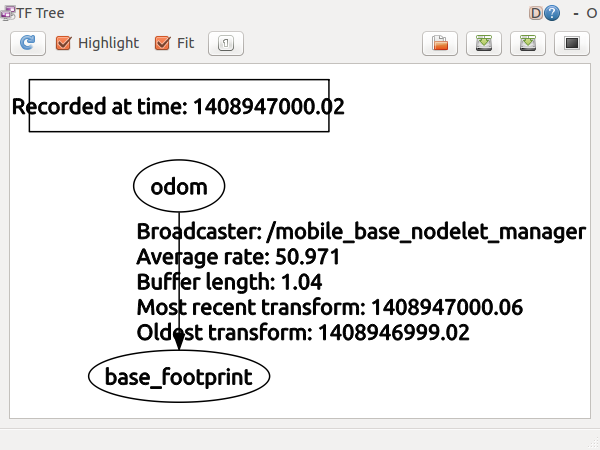
\includegraphics[width=\columnwidth]{pictures/chapter9/pic_09_12.png}
  \caption{tf\_treeによる座標変換の表示}
\end{figure}
\end{lstlisting}

%-------------------------------------------------------------------------------
\section{Kobukiの状態を確認するためのツール}\index{Kobukiの状態を確認するためのツール}

本節では、Kobukiの状態の確認に便利なツールを3つ紹介する。

%-------------------------------------------------------------------------------
\subsection{rqt\_robot\_monitor}

電源やモータ、センサ、処理プログラムなどで生じるエラーメッセージや警告メッセージは、アプリケーション開発には欠くことができない重要な情報である。これらの情報を開発者へ提供するために、ROSでは、rqt\_robot\_monitorパッケージを用意している。次のコマンドでrqt\_robot\_monitorをインストールし、実行する。

\begin{lstlisting}[language=ROS]
$ sudo apt-get install ros-indigo-rqt-robot-monitor
$ rosrun rqt_robot_monitor rqt_robot_monitor
\end{lstlisting}

rqt\_robot\_monitorノードを実行すると、図9-13のように、ロボットに関する様々な情報が表示される。例えばリンクエラーや警告情報、バッテリーの状態、バンパーの状態、落下検知、ホイールドロップ、モータ電流、ジャイロセンサの値、アナログ/デジタル入力値などである。

\begin{figure}[ht]
  \centering
  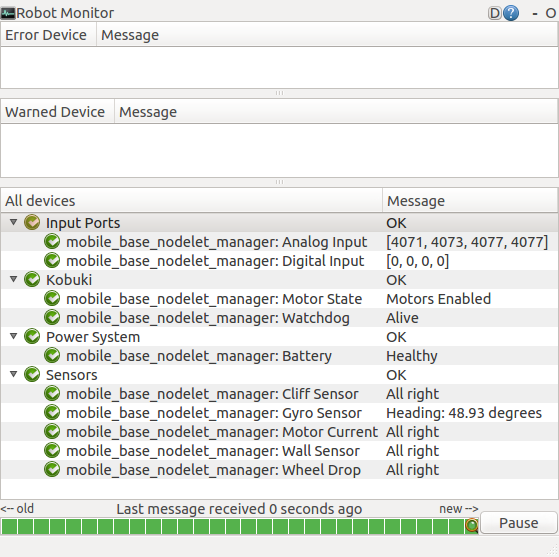
\includegraphics[width=\columnwidth]{pictures/chapter9/pic_09_13.png}
  \caption{rqt\_robot\_monitorを用いたロボットの診断}
\end{figure}

Error Deviceには、ハードウェアやドライバにエラーがある場合に、その内容が表示される。Warned Deviceには、エラーではないが、何か警告すべき状態が生じたときに、その内容が表示される。All devicesにはセンサやバッテリーなどの情報を示される。

ロボットが壁に衝突した場合など、何か問題が発生すると、図9-14のように「Warned Device」の部分に警告マークが表示され、問題の内容が表示される。

\begin{figure}[ht]
  \centering
  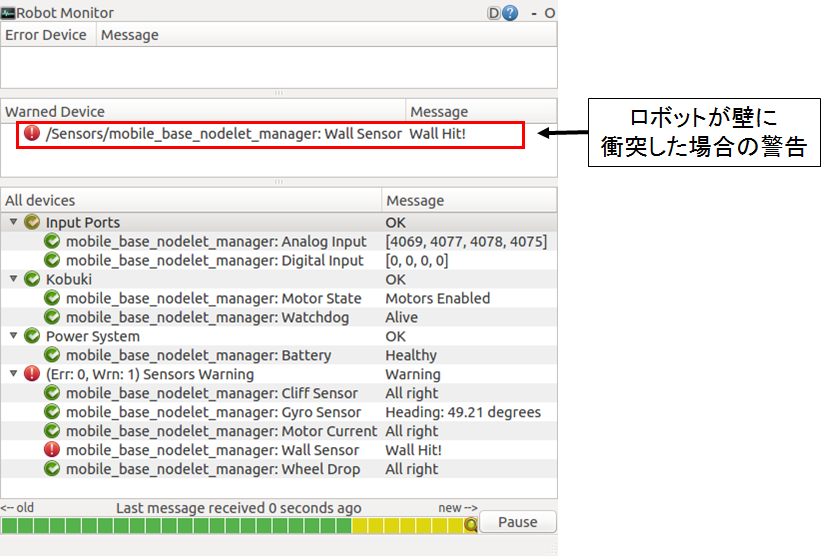
\includegraphics[width=\columnwidth]{pictures/chapter9/pic_09_14.png}
  \caption{ロボットが壁に衝突したときの診断情報}
\end{figure}

%-------------------------------------------------------------------------------
\subsection{ダッシュボード}

Kobukiダッシュボードパッケージ(kobuki\_dashboard)を使うと、前項で   紹介したrqt\_robot\_monitorの情報を含む各種メッセージをGUI形式で確認することができる。例えば、コンソール、モータの状態、LED1とLED2の制御、Kobukiとノートパソコンのバッテリー情報などである。つぎのように関連パッケージをインストールして実行してみよう。

\begin{lstlisting}[language=ROS]
$ sudo apt-get install ros-indigo-kobuki-desktop
$ rosrun kobuki_dashboard kobuki_dashboard
\end{lstlisting}

実行すると、図9-15のように、情報の確認やLEDを制御できるGUI形式のダッシュボードが現れる。

\setcounter{num}{0}
\stepcounter{num}\circled{\thenum} 「Diagnostics   」ボタンをクリックすると、9.7.1項で説明したrqt\_robot\_monitorの情報が追加される。
\stepcounter{num}\circled{\thenum}「Rosout」ボタンをクリックすると、rosoutメッセージが表示される。
\stepcounter{num}\circled{\thenum}「Motors」ボタンをクリックすると、ロボットのモータの電源をOn/Offする。
\stepcounter{num}\circled{\thenum}「LED」ボタンで、KobukiのLED1の状態(Off、緑、オレンジ、赤)を切り替える。
\stepcounter{num}\circled{\thenum}「LED」ボタンで、KobukiのLED2の状態(Off、緑、オレンジ、赤)を切り替える。
\stepcounter{num}\circled{\thenum}「Laptop」はノートパソコンの現在のバッテリー状態を表している。
\stepcounter{num}\circled{\thenum}「Kobuki」はロボットの現在のバッテリー状態を表している。

\begin{figure}[ht]
  \centering
  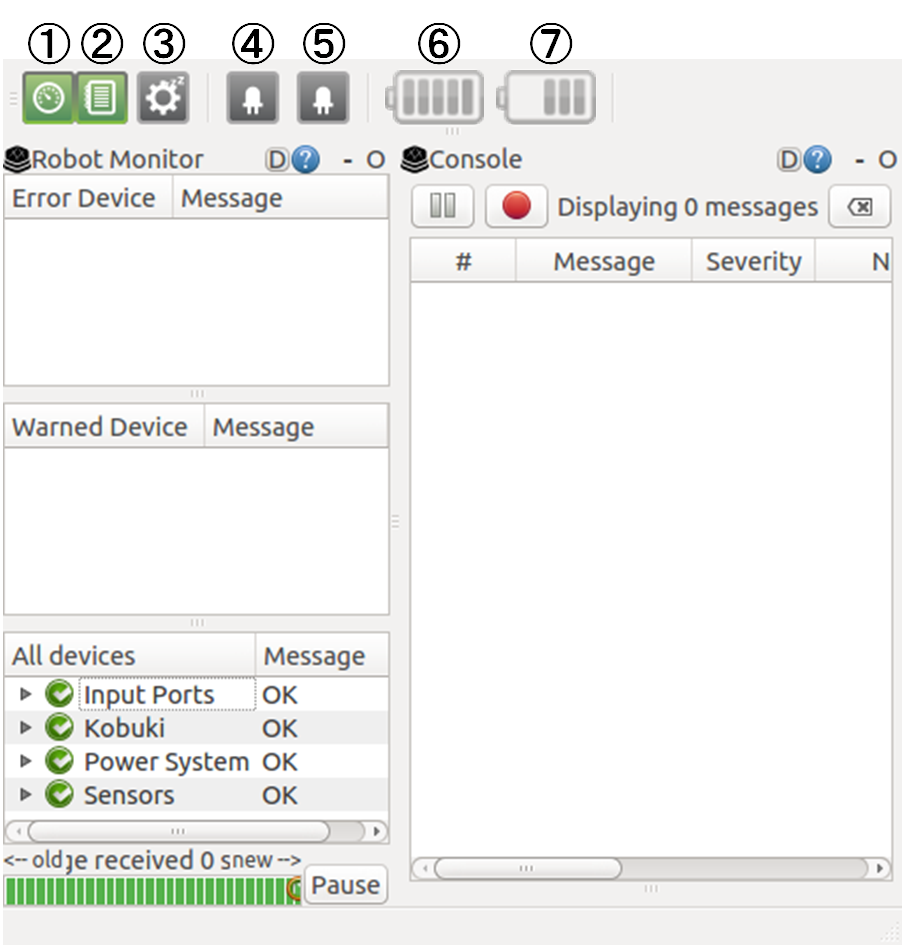
\includegraphics[width=\columnwidth]{pictures/chapter9/pic_09_15.png}
  \caption{ダッシュボード(dashboard)}
\end{figure}

%-------------------------------------------------------------------------------
\subsection{機能テスト(CUI版)}

次に、Kobukiのハードウェアをターミナルウィンドウからテストできるkobuki\_testsuiteパッケージを紹介する。
kobuki\_testsuiteパッケージは、ハードウェアをテストするノードを数多く含むので、Kobukiの故障箇所を把握するのに便利である。使用できるノードには、車輪の回転、イベントの検出、ジャイロテスト、サウンドテスト  などを行うノードがある。これらのノードは表9-7のようにPythonで記述されている。

\begin{table}[h]
\centering
\begin{tabular}{l l}
\toprule
\textbf{ノード名} & \textbf{機能}\\
\midrule
inf\_rotation.py & 車輪を回転させる \\
scan\_angle.py & Kinectを使い前の壁との角度を表示 \\
test\_analog\_input.py  & アナログ入力ポートの4つの値を表示 \\
test\_angular\_acceleration.py  & 回転をしながら角加速度を表示 \\
test\_battery.py & 車輪の回転を繰り返しながらバッテリーの情報をテキストファイルに保存 \\
test\_battery\_voltage.py & バッテリーの情報を表示 \\
test\_digital\_output.py  & 4つのデジタル出力を変更 \\
test\_events.py  & イベント(状態変化)発生の確認 \\
test\_external\_power.py  & 図9-7の外部電源ポットをオン・オフ \\
test\_forwardbackward.py & 前進・後進動作で直進性を確認 \\
test\_gyro.py  & ジャイロセンサ(IMU)で角度、角速度を表示 \\
test\_input.py & 3つのボタン、4つのデジタル入力、2つのバンパー、2つの車輪ドロップセンサ、3つの落下検知センサ、電源入力の状態を表示 \\
test\_led\_array.py & 2つLEDの動作を確認 \\
test\_linear\_acceleration.py & 前進しながら加速度を表示する \\
test\_motion\_forward.py &  前進動作 \\
test\_output.py &  4つの外部電源ポートのオン・オフ、2つのLED、デジタル出力、音などの出力確認 \\
test\_rotation.py  & 回転動作 \\
test\_safewandering.py & 2つのバンパー、3つの落下検知センサを用いて、危険状態における回避動作の確認 \\
test\_slow\_drive.py  & 半径90cmで移動しながらIMU値を表示 \\
test\_sounds.py  & 音のテスト \\
test\_translation.py & オドメトリ、バンパー、IMUなどの情報を表示 \\
\bottomrule
\end{tabular}
\caption{Kobukiの機能テストプログラムの一覧}
\end{table}

必要なノードを実行するには、以下のコマンドを入力する。

\begin{lstlisting}[language=ROS]
rosrun kobuki_testsuite %*ノード名*)
\end{lstlisting}

以下は「test\_events.py」を実行した例である。イベント  (状態変化)を発生させるために、最初に右のバンパーを押し、離した後、ロボットを床上に置いた。バンパー、ホイールドロップ、落下検知センサが反応して、イベントが発生することが確認できる。

\begin{lstlisting}[language=ROS]
$ rosrun kobuki_testsuite test_events.py
Try kobuki's hardware components; the following events should be reported:
- buttons
- bumpers
- wheel drops
- cliffs
- plug/unplug adapter
- dock/undock on base
- charge completed
- battery low/critical
- digital input changes
[INFO] [WallTime: 1408952137.104793] Right bumper is pressed.
[INFO] [WallTime: 1408952137.185717] Right bumper is released.
[INFO] [WallTime: 1408952140.866974] Left wheel is dropped.
[INFO] [WallTime: 1408952140.886718] Right wheel is dropped.
[INFO] [WallTime: 1408952141.127440] Right side of robot is on the cliff.
[INFO] [WallTime: 1408952141.207462] Left side of robot is on the cliff.
[INFO] [WallTime: 1408952141.210328] Centre side of robot is on the cliff.
[INFO] [WallTime: 1408952141.627020] Left side of robot is on the floor.
[INFO] [WallTime: 1408952141.668215] Centre side of robot is on the floor.
[INFO] [WallTime: 1408952141.726817] Right side of robot is on the floor.
[INFO] [WallTime: 1408952141.807727] Left wheel is raised.
[INFO] [WallTime: 1408952141.847553] Right wheel is raised.
\end{lstlisting}

%-------------------------------------------------------------------------------
\section{Kobukiファームウェアのアップグレード}\index{Kobukiファームウェアのアップグレード}

Kobukiのファームウェアは、Kobukiを制御するための最も基本的なソフトウェアである。ファームウェアは工場出荷時にKobukiにインストールされているが、バグの修正などメーカにより更新されるので、自分で最新のものをインストールする必要がある。最新のファームウェアのバージョンはYujin Robot社のホームページ(http://files.yujinrobot.com/kobuki/firmware/)から確認できる。2015年8月現在の最新のバージョンは1.2.0である。

%-------------------------------------------------------------------------------
\subsection{ファームウェアのバージョンの確認}

Kobukiのファームウェアのバージョンを確認する方法は2つある。一つは、kobuki\_nodeを実行するときに「--screen」オプションを付ける方法であり、もう一つはkobuki\_nodeを実行した後に「/mobile\_base/version\_info」トピックを調べる方法である。以下で具体的にみてみよう。
次のようにroslaunchコマンドの最後に「--screen」オプションを付けると、ノードが実行されるのと同時に、ファームウェアのバージョンを確認できる。

\begin{lstlisting}[language=ROS]
$ roslaunch kobuki_node minimal.launch --screen
[INFO] [1408612929.814111512]: Kobuki : Version info - Hardware: 1.0.4. Firmware: 1.1.4
\end{lstlisting}

この場合、「Firmware:」に続く数字「1.1.4」がバージョンである。
kobuki\_nodeが配信するトピックからファームウェアのバージョンを確認する方法を、次に示す。

\begin{lstlisting}[language=ROS]
$ rostopic echo /mobile_base/version_info
hardware: 1.0.4
firmware: 1.1.4
software: 0.6.0
udid: [98107192, 825317169, 1460173122]
features: 3
---
\end{lstlisting}

%-------------------------------------------------------------------------------
\subsection{ファームウェアバージョンの更新}

ファームウェアのバージョンを確認して古いことがわかったら、以下の手順で更新をおこなう。まず、Kobukiのファームウェア注4ファイルhex注5と、これをKobukiにアップロードするためのstm32flash注6プログラムをダウンロードし、stm32flashプログラムを makeして実行可能な状態にしておく。

\begin{lstlisting}[language=ROS]
$ mkdir ~/firmware_update
$ cd ~/firmware_update
$ wget http://stm32flash.googlecode.com/files/stm32flash.tar.gz
$ wget http://files.yujinrobot.com/kobuki/firmware/kobuki_firmware-latest.hex
$ tar -xvf stm32flash.tar.gz
$ cd stm32flash
$ make
\end{lstlisting}

次に、Kobukiのファームウェアをアップグレードする具体的な手順を示す。まず   Kobukiの電源を切り、次に図9-16のようにファームウェアのダウンロード受信機能の切り替えスイッチを「Download」に設定し、再び電源を入れる。起動後、次のコマンドを入力することで、ファームウェアファイルがKobukiにアップロードされ、更新される。

\begin{lstlisting}[language=ROS]
$ ./stm32flash -b 115200 -w ../kobuki_firmware-latest.hex /dev/ttyUSB0
\end{lstlisting}

ただしオプションとして「/dev/ttyUSB0」のようにポートを指定したが、これはユーザーごとに異なるので、9.5節に示したように、以下の方法で確認してほしい。

\begin{lstlisting}[language=ROS]
$ ls -l /dev/kobuki
lrwxrwxrwx 1 root root 7 Aug 24 14:26 /dev/kobuki -> ttyUSB0
\end{lstlisting}

\begin{figure}[ht]
  \centering
  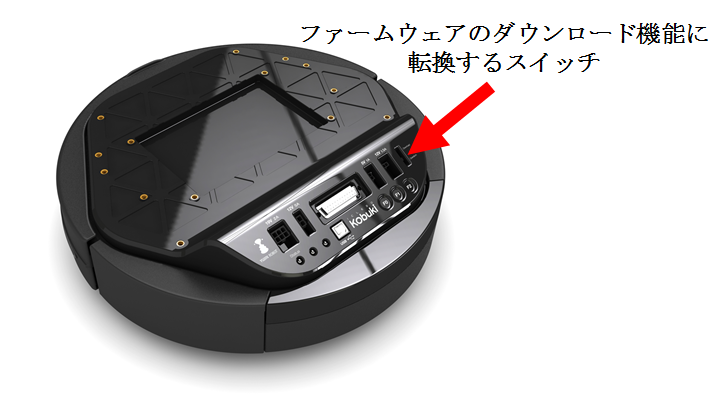
\includegraphics[width=\columnwidth]{pictures/chapter9/pic_09_16.png}
  \caption{ファームウェアのダウンロード受信機能切り替えスイッチ}
\end{figure}

ファームウェアの更新が完了したら、Kobukiのダウンロード受信機能の切り替えスイッチを元の状態に戻し、Kobukiを再起動する。ファームウェアの更新が正常に行われたことを確認するには、前述したファームウェアのバージョン確認方法のいずれかを実行すればよい。例えば、次のようにファームウェアが最新バージョンに更新されたことが確認できる  。

\begin{lstlisting}[language=ROS]
$ roslaunch kobuki_node minimal.launch --screen
[INFO] [1408953316.298156409]: Kobuki : Version info - Hardware: 1.0.4. Firmware: 1.2.0
\end{lstlisting}

%-------------------------------------------------------------------------------
\section{Kobukiの自動ドッキング}\index{Kobukiの自動ドッキング}

本節では、ドッキングステーションとKobukiの接続について、自動的にドッキングするためのパッケージや具体的なアルゴリズムを紹介する。

  %-------------------------------------------------------------------------------
  \subsection{Kobukiとドッキングステーション}

Kobukiが自走してバッテリーを充電するには、図9-8のドッキングステーションが必要である。ドッキングステーションは、充電アダプタを内部に含んでおり、図9-17に示す下部の充電端子を介してロボットと接続すると充電を開始する。K obukiとドッキングステーションのドッキングに使用されるハードウェアは、ドッキングステーション側の3つのIR(赤外線)発光部(中央、左、右)と3つのKobuki本体側の受光部、充電端子と充電状態表示LEDである。

\begin{figure}[ht]
  \centering
  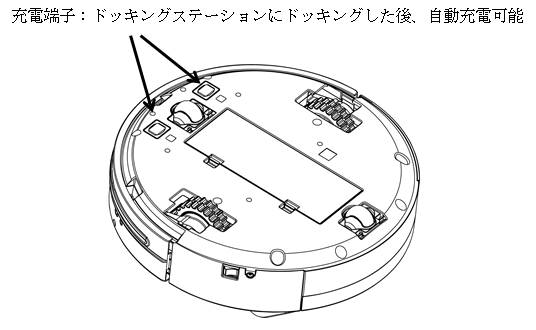
\includegraphics[width=\columnwidth]{pictures/chapter9/pic_09_17.png}
  \caption{Kobuki本体の充電端子}
\end{figure}

%-------------------------------------------------------------------------------
\subsection{ドッキングおよび自動充電}

ドッキングと自動充電には、kobuki\_auto\_docking注7パッケージを使用する。以下のコマンドでminimal.launchノードを実行する。

\begin{lstlisting}[language=ROS]
$ roslaunch kobuki_node minimal.launch --screen
\end{lstlisting}

つぎに、さらに別のドッキング関連ノードを実行する。

\begin{lstlisting}[language=ROS]
$ roslaunch kobuki_auto_docking minimal.launch --screen
\end{lstlisting}

なお、次のlaunchファイルを利用すれば、これら2つのノードを一度に起動できる。

\begin{lstlisting}[language=ROS]
$ roslaunch kobuki_auto_docking compact.launch --screen
\end{lstlisting}

次のコマンドでドッキングが開始される。Kobukiはドッキングステーションを探索して、ドッキングステーションの正面に移動  し、結合する。その後、自動的に充電状態になる。

\begin{lstlisting}[language=ROS]
$ roslaunch kobuki_auto_docking activate.launch --screen
\end{lstlisting}

図9-18に自動ドッキングの様子を示す。

\begin{figure}[ht]
  \centering
  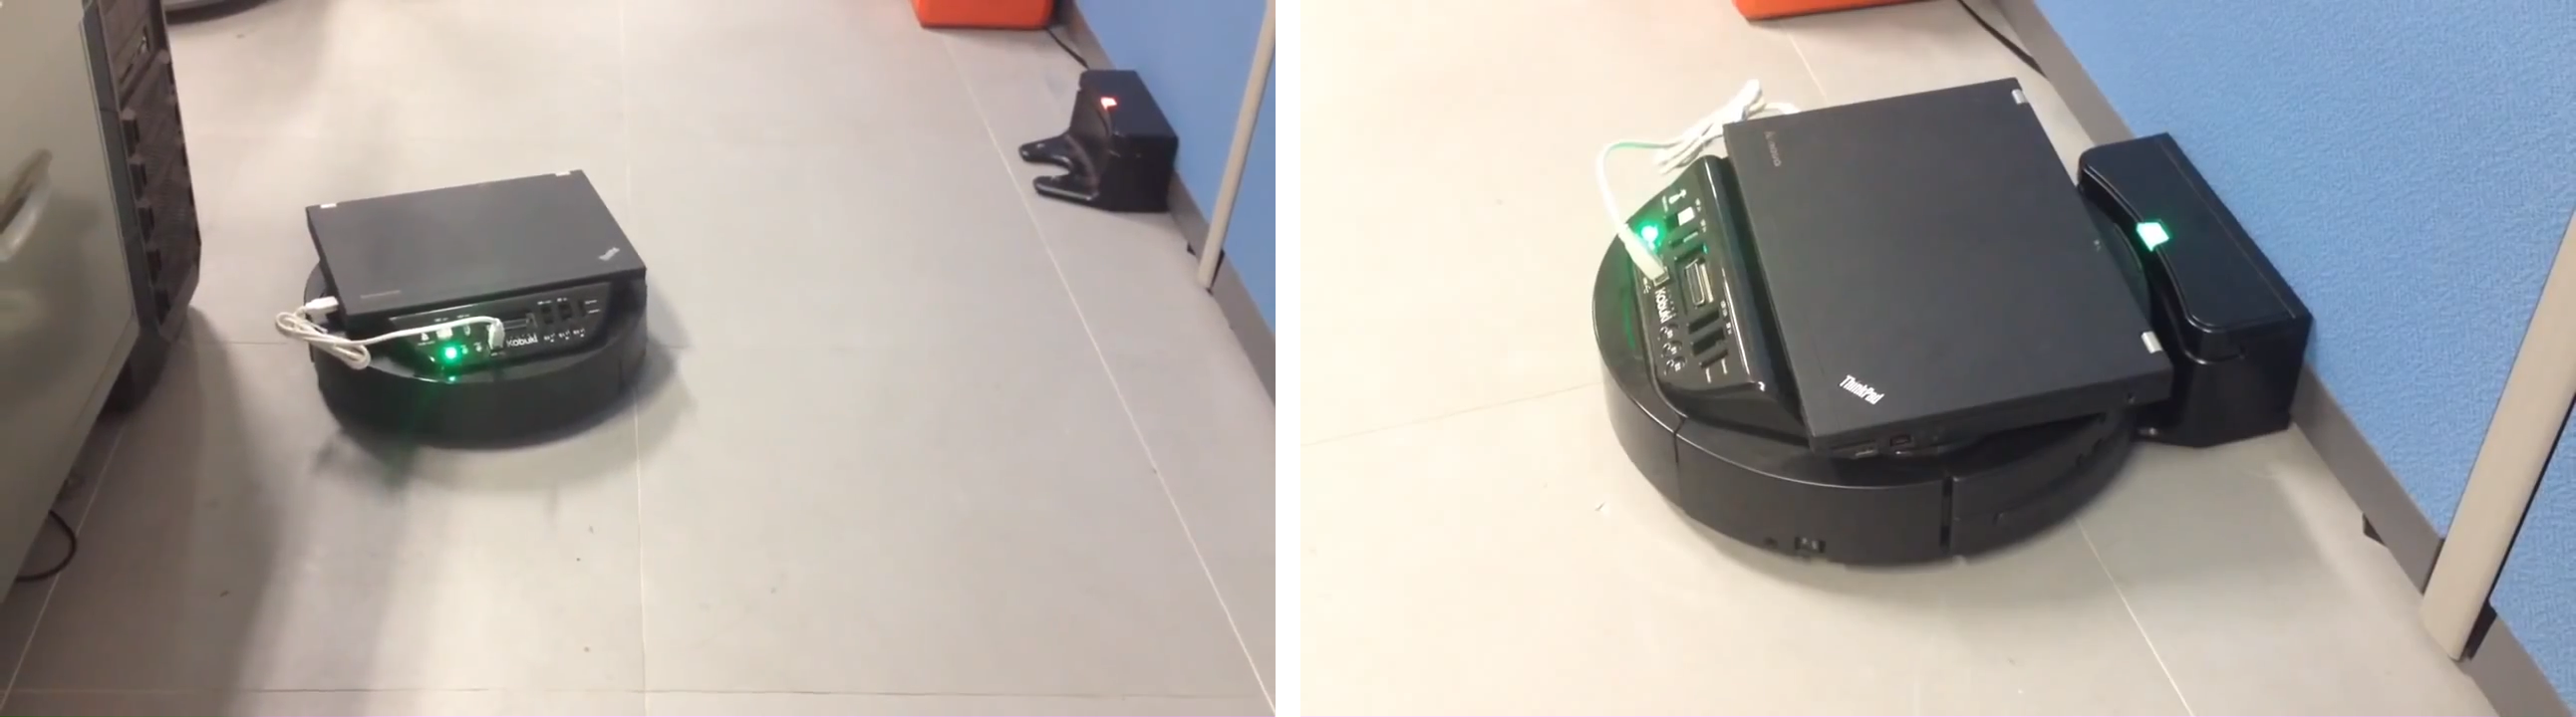
\includegraphics[width=\columnwidth]{pictures/chapter9/pic_09_18.png}
  \caption{ドッキングおよび自動充電の様子}
\end{figure}

\begin{exercise}[Kobukiとドッキングステーションの状態表示LED]

  状態表示LED(Status LED)は、Kobukiの制御パネルの左端にあり、Kobukiの現在のバッテリーの状態を表す。

  \begin{itemize}
  \item 緑: バッテリー残量が十分であることを示す。
  \item オレンジ: バッテリー残量が低いことを示す(充電が必要な状態)。
  \item 緑点滅: バッテリーが充電中であることを示す。
  \end{itemize}

  ドッキングステーションの充電状態表示LEDは、現在の充電状態を表す。

  \begin{itemize}
  \item 赤: Kobukiがドッキングされていない。
  \item 緑点滅: Kobukiがドッキングされており、充電中である。
  \item 緑: Kobukiがドッキングされており、充電が完了した状態である。
  \end{itemize}
\end{exercise}

%-------------------------------------------------------------------------------
\subsection{ドッキングアルゴリズム}

Yujin Robot社では、参考資料注8でKobukiの自動ドッキングに関連する  プログラム注9を公開している。
まず、ドッキングステーションの赤外線発光部は、図9-8のように左、中央、右の合計3箇所にある。そこで、ドッキングステーションの前の領域を、図9-19に示すように、左、中央、右の3つの領域に分け、さらに距離に応じて   これを近距離、遠距離の2つに分ける  。したがって、Kobukiとドッキングステーションの位置には、以下の7つのパターンがある。0~32までの数字はそれぞれの状態の番号、()はその16進数での値である。近距離と遠距離で両方検出された場合(例えばNEAR\_LEFT+FAR\_LEFT=0x11)には、近距離が優先される。

\begin{itemize}[leftmargin=*]
\item NONE = 0  (=0x00)
\item NEAR\_LEFT = 1 (=0x01)
\item NEAR\_CENTER = 2 (=0x02)
\item NEAR\_RIGHT = 4 (=0x04)
\item FAR\_LEFT = 16 (=0x10)
\item FAR\_CENTER = 8 (=0x08)
\item FAR\_RIGHT = 32 (=0x20)
\end{itemize}

\begin{figure}[ht]
  \centering
  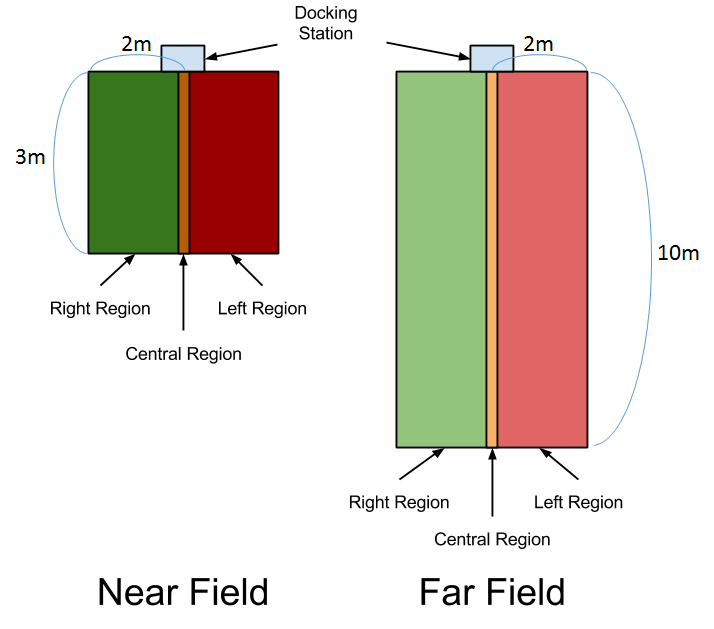
\includegraphics[width=\columnwidth]{pictures/chapter9/pic_09_19.png}
  \caption{ドッキングステーションの領域}
\end{figure}

図9-20に示すように、Kobuki本体には3つの受光部があり、それぞれドッキングステーションの赤外線発光部からの赤外線を受光できる。もしKobukiがドッキングステーションの赤外線を受光できる領域内にある場合、kobuki\_auto\_dockingノードが実行可能である。受光可能な領域は、ドッキングステーションを中心に水平2m、垂直正面方向に5m程度   である。Kobukiは、ドッキングのために所定の位置で回転し、3つの赤外線受光部のいずれかで赤外線を検出すると、ドッキング作業を実行する。

\begin{figure}[ht]
  \centering
  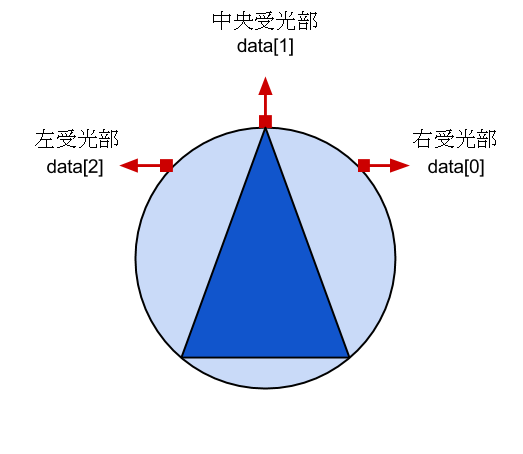
\includegraphics[width=\columnwidth]{pictures/chapter9/pic_09_20.png}
  \caption{赤外線受信部の位置と方向}
\end{figure}

以下は、トピックを利用してドッキングに関するセンサ情報を確認するコマンドである。

\begin{lstlisting}[language=ROS]
$ rostopic echo /mobile_base/sensors/dock_ir
---
header:
 seq: 17202
 stamp:
  secs: 1408965261
  nsecs: 393052992
 frame_id: dock_ir_link
data: [0, 0, 32]  %* [右受光部、中央受光部、左受光部]*)
---
\end{lstlisting}

この例では、現在、Kobukiの左の左受光部は32(=FAR\_RIGHT)の状態であり  、これはKobukiの左の左受光部がドッキングステーションの右側の領域内の遠い場所にいることを意味する。したがって、この場合にはドッキングステーションはKobukiの左側の遠い位置にあることがわかる。
このように  Kobukiは、ドッキングステーションの赤外線発光部とKobuki本体の赤外線受光部を利用して相対位置を検出し、自動的にドッキングを行うが、その流れは次の3つのパターン   のいずれかとなる。

\begin{enumerate}[leftmargin=*]
\item Kobukiがドッキングステーションの正面にあるとき、ドッキング充電端子に触れるまで、まっすぐ直進してドッキングする。

\item Kobukiがドッキングステーションの左側にあるとき、Kobukiの右の右受光部がドッキングステーションの左側の赤外線発光部を検出  するまで、反時計回りに回転する。左側の赤外線発光部を検出すると、ドッキングステーションの正面まで直進する。その後、時計回りに回転して、Kobukiの中央受光部がドッキングステーション中央の赤外線発光部を検出すると、直進してドッキングする。

\item Kobukiが右にある場合も、方向が違うだけで、2と同様のアルゴリズムで動作する。
\end{enumerate}

現在ドッキングアルゴリズムは、ドッキングステーションからの赤外線が受光可能な領域の外にKobukiが置かれるとドッキングができないこと   や、ドッキングまでの時間が長いことなど、改善の余地がある。興味のある読者は、新しいドッキングアルゴリズムを提案してみるのもいい。

%-------------------------------------------------------------------------------
\section{RVizを利用したKobukiシミュレーション}\index{RVizを利用したKobukiシミュレーション}

Kobukiでは、仮想ロボットを利用したシミュレーションによるプログラミング開発が可能である。その方法は2つあり、1つはROSの3次元可視化ツールであるRVizを利用する方法、もう1つは3次元ロボットシミュレータGazeboを用いる方法である。これらの可視化ツールやシミュレータ  を使えば、Kobuki本体がなくても、独自にパッケージの開発・評価ができる。本節では、RVizを利用し、Kobukiが指定された経路上を移動するシミュレーションについて説明する。
なお、RVizでは、動作指令に応じたKobukiの動作はシミュレーションできるが、動力学的な情報や外界センサの情報は再現できない。これらの情報を利用するには、物理エンジンを有する3次元シミュレータGazeboを用いる必要がある。Gazeboについては次節で説明する。

%-------------------------------------------------------------------------------
\subsection{シミュレーションの準備}

RVizによるKobukiのシミュレーションを実行するには、kobuki\_soft注10メタパッケージを利用する。

\subsubsection{kobuki\_soft(メタパッケージ)}

\begin{itemize}
\item wiki: http://wiki.ros.org/kobuki\_soft
\item リポジトリ: https://github.com/yujinrobot/kobuki\_soft
\end{itemize}

kobuki\_softは、RViz環境でモータを仮想的に制御してKobukiの動作を再現するものである。このメタパッケージに含まれるパッケージを以下に示す。

\subsubsection{kobuki\_softnode}

\begin{itemize}
\item wiki: http://wiki.ros.org/kobuki\_softnode
\item 機能: RVizで実行可能なKobukiのシミュレーション環境を提供する基本パッケージである。
\end{itemize}

\subsubsection{kobuki\_softapps}

\begin{itemize}
\item wiki: http://wiki.ros.org/kobuki\_softapps
\item 機能: kobuki\_softnodeの関連パッケージで、主にナビゲーション機能を提供する。
\end{itemize}

シミュレーションの準備として、まずkobuki\_softパッケージをインストールする。

\begin{lstlisting}[language=ROS]
$ sudo apt-get install ros-indigo-kobuki-soft
\end{lstlisting}

%-------------------------------------------------------------------------------
\subsection{仮想Kobukiの準備}

シミュレーションで仮想的にKobukiを利用するには、次のコマンドでkobuki\_softnodeパッケージのfull.launchファイルを実行する。

\begin{lstlisting}[language=ROS]
$ roslaunch kobuki_softnode full.launch --screen
\end{lstlisting}

これにより、kobuki\_descriptionパッケージでKobukiの3次元モデルが読み込まれ、kobuki\_nodeパッケージと同様の様々なノード(mobile base nodelet manager、mobile base、diagnostic aggregator、robot state publisher)が仮想的に利用できる。
これらのノードは、turtle\_teleop\_keyノードから配信されるvelocity、motor\_powerなどのモータ駆動命令を購読し、仮想的にモータを駆動してKobukiを制御する。例えば、mobile\_baseノードは、速度コマンドを受け取り、オドメトリ情報を計算し、自己位置に関するトピックを配信する。また同時
にjoint statesやtfなどのトピックも配信しており、RVizでKobukiの動きをシミュレーションにより確認できる。

次に、RVizを実行して、左のディスプレイウィンドウで[Global Options]→[fixed frame]を「/odom」に変更  する。そして、ディスプレイウィンドウの左下の<Add>ボタンを押して、「RobotModel」を選択して追加する。すでにfull.launchファイルでKobukiの3次元モデルを読み込んだので、図9-21のようにそのモデルが画面中央に表示される。

\begin{figure}[ht]
  \centering
  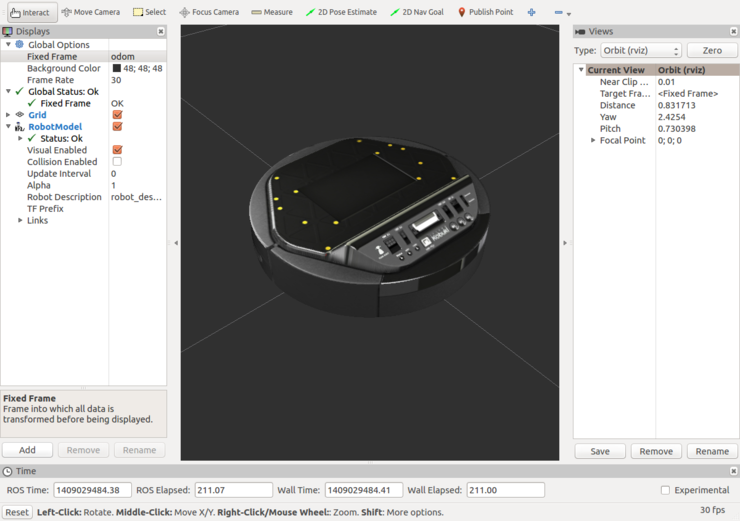
\includegraphics[width=\columnwidth]{pictures/chapter9/pic_09_21.png}
  \caption{仮想ロボットの実行}
\end{figure}

次に、keyop.launchファイルを実行して、仮想のKobukiの動作をキーボードで制御してみよう。

\begin{lstlisting}[language=ROS]
$ roslaunch kobuki_keyop keyop.launch
\end{lstlisting}

キーボードの矢印を押すと、仮想のKobukiがRVizの画面内を移動することが確認できる。

\subsubsection{odomトピックの確認}

仮想のKobukiの動作を確認した  ので、続いて、オドメトリ情報が正しく計算され、配信されているかを確認する。rostopic echo /odom コマンドでも確認できるが、今回はRVizを用いているので、GUI環境で視覚的に確認してみる。RVizの左下の<Add>ボタンを押して、図9-22のように「By Topic」タブをクリックし、「Odometry」を選択する。これにより、画面上のKobukiの前進方向に、オドメトリを示す赤い矢印が現れる。初期設定ではこの矢印が長すぎるので、左側のディスプレイウィンドウの[Odometry]詳細オプションで「Length」の値を0.5に設定する。
次に、再び「keyop.launch」ノードを使用して仮想のKobukiを動かすと、図9-23のように、Kobukiの軌跡に沿って赤い矢印が表示されることが確認できる。このオドメトリ情報は、移動ロボットの推定位置を示す。

\begin{figure}[ht]
  \centering
  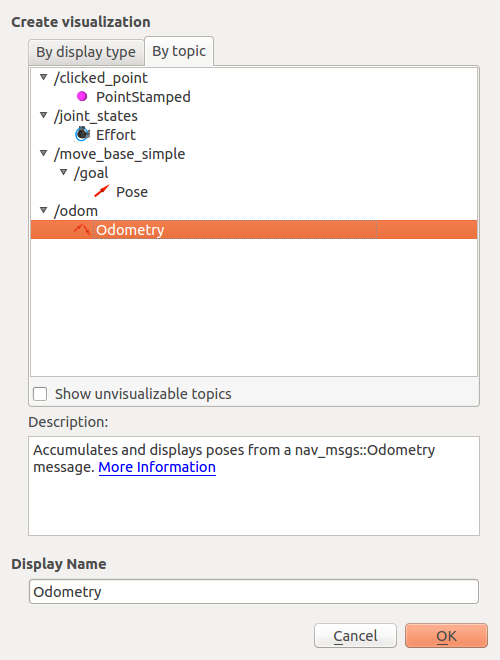
\includegraphics[width=\columnwidth]{pictures/chapter9/pic_09_22.png}
  \caption{odomトピックの確認のためodometryディスプレイを追加}
\end{figure}

\begin{figure}[ht]
  \centering
  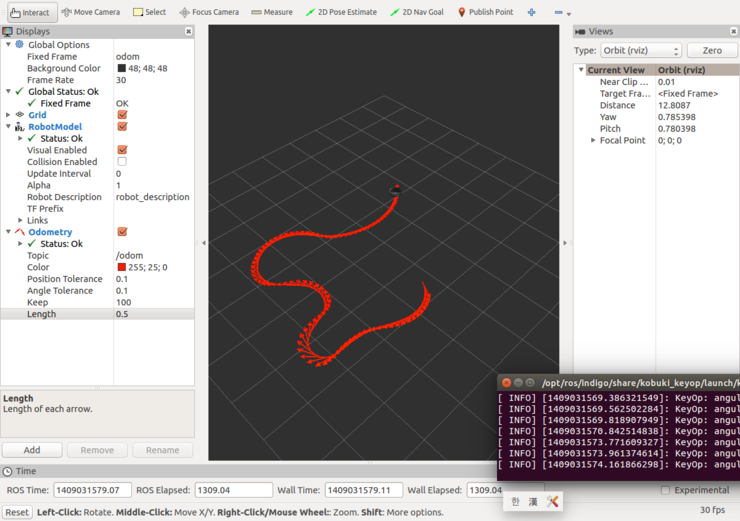
\includegraphics[width=\columnwidth]{pictures/chapter9/pic_09_23.png}
  \caption{keyop.launchを利用した仮想ロボットの制御}
\end{figure}

\subsubsection{tfトピックの確認}

オドメトリ情報(odomトピック)のつぎに、Kobukiを構成する部品  の相対位置を含むtfトピックの確認方法を学ぼう.これは、rostopicコマンドを使って確認することもできるが、ここではodomと同様にRVizを利用して確認し、階層構造はrqt\_tf\_treeにより表示してみる。
RVizの左下の<Add>ボタンを押して「TF」を選択する。すると、図9-24のようにodom、base\_footprint、gyro\_link、wheel\_left\_link、wheel\_right\_linkなどが表示される。ここで再び「keyop.launch」を利用して、仮想のKobukiを動かしてみよう。Kobukiが移動すると、左右の車輪を表すwheel\_left\_link、wheel\_right\_linkのtfマークが回転する。
次にrqt\_tf\_treeを実行する。これにより、図9-25のように各部品  の相対位置関係が確認できる。同様に、ロボットにセンサを取り付けた場合、その取り付け位置も各部品と同様にtfで表現することができる。tfについては10.3節で詳細に説明する。

\begin{lstlisting}[language=ROS]
$ rosrun rqt_tf_tree rqt_tf_tree
\end{lstlisting}

\begin{figure}[ht]
  \centering
  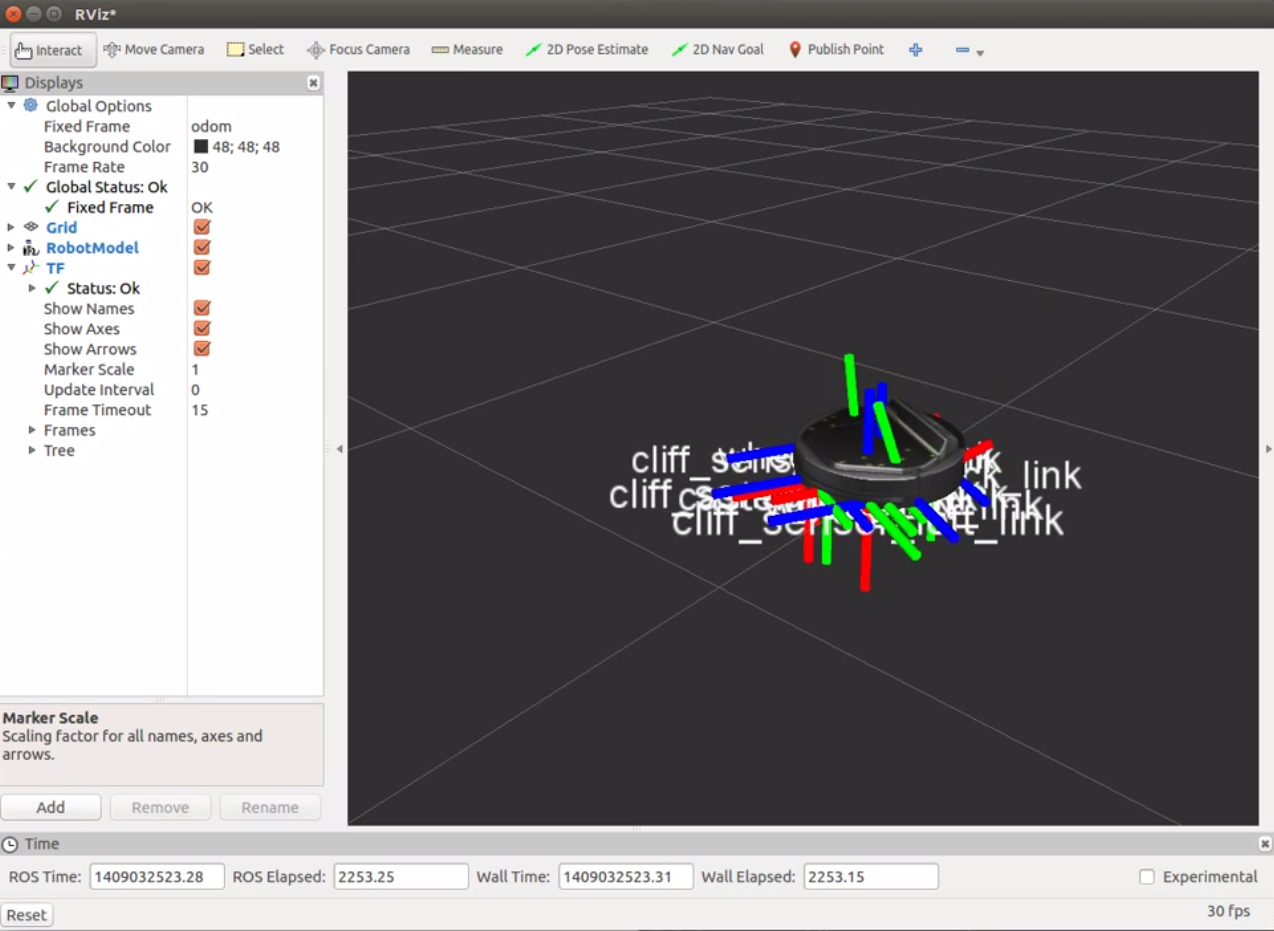
\includegraphics[width=\columnwidth]{pictures/chapter9/pic_09_24.png}
  \caption{RVizを用いたtfトピックの確認}
\end{figure}

\begin{figure}[ht]
  \centering
  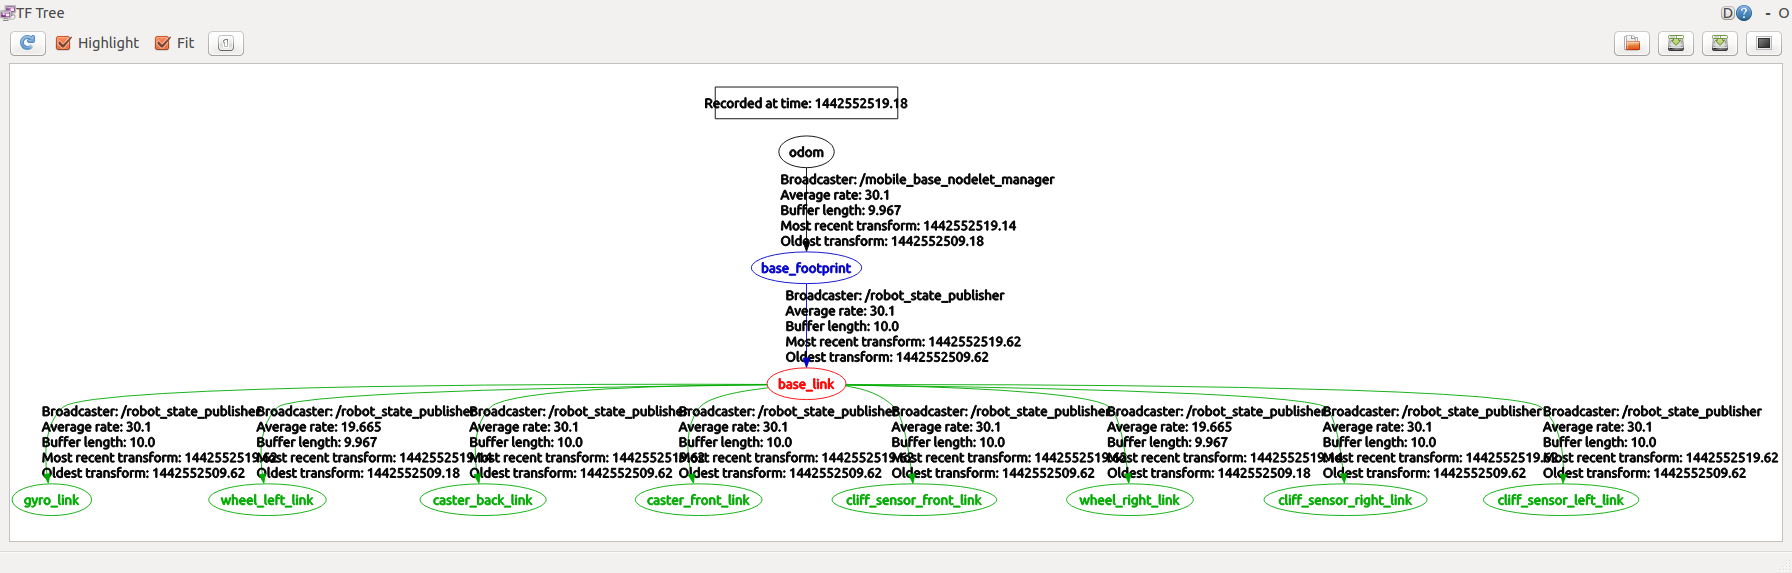
\includegraphics[width=\columnwidth]{pictures/chapter9/pic_09_25.png}
  \caption{rqt\_tf\_treeを用いたtfトピックの確認}
\end{figure}

%-------------------------------------------------------------------------------
\subsection{仮想ナビゲーション}

ナビゲーションとは、指定された目標位置にロボットを移動させる技術である。実際のKobukiのナビゲーションについては、10章で説明する。本項では、仮想のKobukiのナビゲーションを説明する。
kobuki\_softパッケージには、仮想ナビゲーションに必要な環境が含まれているが、これを使用するには、さらにいくつかのパッケージをインストールする必要がある。本項では、ROSの代表的なパッケージであるnavigationと、YujinRobot社のyujin-mapsをインストールする。

\begin{lstlisting}[language=ROS]
$ sudo apt-get install ros-indigo-navigation ros-indigo-yujin-maps
\end{lstlisting}

次に、実行中のroscore以外のすべてのノードを<Ctrl> + <c>で終了し、次のコマンドを実行する。

\begin{lstlisting}[language=ROS]
$ roslaunch kobuki_softapps nav_demo.launch
\end{lstlisting}

これにより、図9-26のようにRVizが自動的に起動するが、これにはナビゲーションに必要な環境があらかじめ含まれている。RViz画面上の<2D Nav Goal>アイコンを選択して、地図上の任意の位置をクリック、ドラッグして、目標位置と目標姿勢  を設定してみよう。仮想のKobukiが障害物を避けて、目標位置、姿勢まで移動する様子が確認できる。

\begin{figure}[ht]
  \centering
  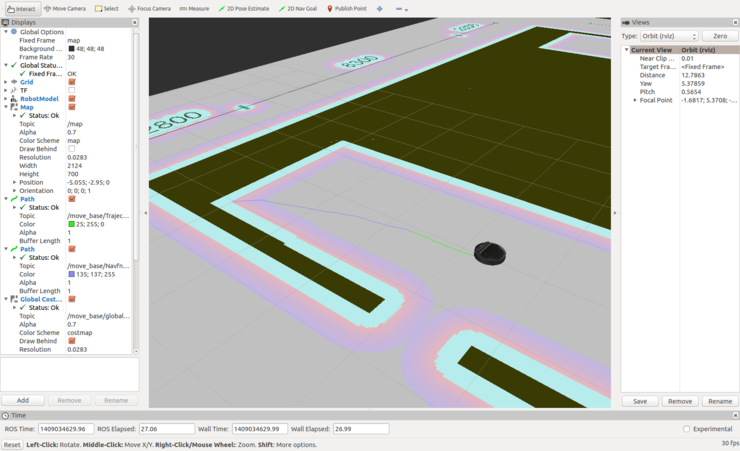
\includegraphics[width=\columnwidth]{pictures/chapter9/pic_09_26.png}
  \caption{nav\_demo.launchの実行画面}
\end{figure}

\begin{exercise}[nav\_demo.launchの問題点]
kobuki\_softapps パッケージは、RViz環境でのオドメトリ情報とモータのシミュレーションを目的としており、外界センサから得られる環境情報は再現できないため、障害物に衝突する場合がある。外界センサも再現するには、stageやgazeboなどの別のシミュレーション環境が必要となる。
\end{exercise}

%-------------------------------------------------------------------------------
\section{Gazeboを利用したKobukiシミュレーション}\index{Gazeboを利用したKobukiシミュレーション}

%-------------------------------------------------------------------------------
\subsection{Gazeboとは}

Gazebo注11 は、物理エンジンを搭載したロボットアプリケーション開発のための3次元シミュレータである。OSRFで開発されたオープンソースシミュレータ注12の中でも高い評価を受けており、米国DARPA Robotics Challenge注13の公式シミュレータに選定されるなど、開発が加速している。ROSも、Player/Stage、Gazeboを基本シミュレータとして推奨しており、ROSへの導入も容易である注14。

Gazeboの特徴は次の通りである。

\begin{itemize}
\item 様々な物理エンジンによる動力学シミュレーション  : 物理エンジンには、開発当初のGazeboはODE注15のみをサポートしていたが、バージョン3.0  以降では、ユーザーのさまざまな要求に応えるため、Bullet注16、Simbody注17、DART注18など、多くの物理エンジンが選択できるようになっている。
\item 高度な 3次元グラフィックス機能: Gazeboでは、3次元グラフィクスエンジンにOGRE(open-source graphics rendering engines)注19を採用し、高度なレンダリング機能を提供している。
\item  多様なセンサ:  LRF、カメラ、デプスカメラ、接触センサ、力-トルクセンサなど、多くの内界、外界センサを再現できる。さらに、検出されたセンサデータへのノイズの付加も可能である。
\item  プラグインによる機能拡張: プラグイン開発のためのAPI注20が提供され、ユーザーはロボットやセンサ、制御プログラムなどの独自のプラグインを開発、導入できる。
\item  多様なロボットモデル: PR2、Pioneer2 DX、iRobot Create、TurtleBotなど市販の多くのロボットが、GazeboのモデルファイルであるSDF(Simulated Description Format)注21形式で提供されている。独自のロボットも追加できる。
\item  リモートサーバー機能の提供: ソケットベースのメッセージパッシングであるグーグルプロトバッファ(Protobufs)注22を利用して、リモートサーバーでもシミュレーションが実行可能である  。
\item  クラウドシミュレーションの提供: GazeboをAmazon、Softlayer、OpenStackなどで使用できるよう、CloudSim注23を使用したクラウドシミュレーション環境を提供している。
\item コマンドラインツール: 豊富なコマンドラインツール  を利用して、シミュレーションの状態を把握、制御することができる。
\end{itemize}

%-------------------------------------------------------------------------------
\subsection{Gazeboのインストール}

2015年8月時点で、Gazeboの最新バージョンは6.0である  。しかしROSコミュニティでは、ROSのIndigoバージョンでは  バージョン2.2を推奨  しており、本書でもバージョン2.2を使用する。
まず、次のようにモデル処理パッケージsdformatとgazebo2をインストールしよう。gazebo2をインストールすると、バージョン2.2がインストールされる。

\begin{lstlisting}[language=ROS]
$ sudo sh -c 'echo "deb http://packages.osrfoundation.org/gazebo/ubuntu trusty main" > /etc/ apt/sources.list.d/gazebo-latest.list'
$ wget http://packages.osrfoundation.org/gazebo.key -O - | sudo apt-key add -
$ sudo apt-get update
$ sudo apt-get install libsdformat1 libsdformat-dev gazebo2
\end{lstlisting}

次に、以下のようにGazeboを実行すると、図9-27のようにGazeboの初期画面が表示される。

\begin{lstlisting}[language=ROS]
$ gazebo
\end{lstlisting}

\begin{figure}[ht]
  \centering
  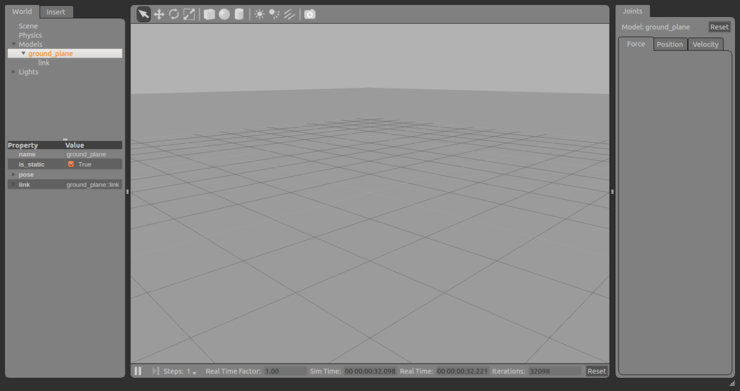
\includegraphics[width=\columnwidth]{pictures/chapter9/pic_09_27.png}
  \caption{Gazeboの初期画面}
\end{figure}

次に、GazeboシミュレータでのKobukiの動作に関連するパッケージをインストールする。関連パッケージは様々あるが、ここでは、GazeboとROSを連携させるgazebo\_ros\_pkgsメタパッケージ、Kobukiの3次元シミュレーションのためのkobuki\_desktopメタパッケージを導入する。

\begin{lstlisting}[language=ROS]
$ sudo apt-get install ros-indigo-gazebo-ros ros-indigo-gazebo-plugins ros-indigo-kobuki-desktop
\end{lstlisting}

%-------------------------------------------------------------------------------
\subsection{GazeboによるKobukiシミュレーション}

では、実際にGazeboを用いてKobukiの動作をシミュレーションしてみる。ただし、図9-27が表示されている場合には、Gazeboを終了しておく。 では、次のlaunchファイルを実行してみよう。

\begin{lstlisting}[language=ROS]
$ roslaunch kobuki_gazebo kobuki_empty_world.launch
\end{lstlisting}

これにより、gazebo、gazebo\_gui、mobile\_base\_nodelet\_ manager、robot\_state\_publisher、spawn\_mobile\_baseノードが一斉に起動され、図9-28のようにKobukiがGazeboの画面に現れる。

\begin{figure}[ht]
  \centering
  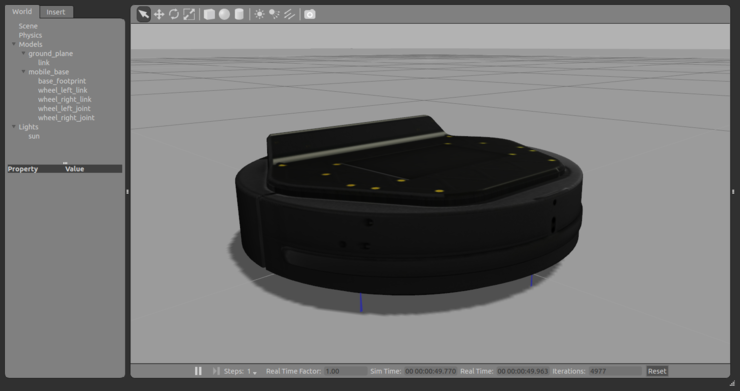
\includegraphics[width=\columnwidth]{pictures/chapter9/pic_09_28.png}
  \caption{gazebo上kobukiの3次元外観}
\end{figure}

次に、kobuki\_keyopファイルを実行すると、Gazebo環境で仮想のKobukiが制御できる。

\begin{lstlisting}[language=ROS]
$ roslaunch kobuki_keyop keyop.launch
\end{lstlisting}

次に、初期設定である床のモデルground\_planeとKobukiのモデルmobile\_baseに加え、テーブル6個、コンクリートブロック3つをgazebo画面の「insert」タップから選択   し、追加する。追加後のGazeboの環境モデルを記述したworldファイルは、以下に置かれている。

\begin{lstlisting}[language=ROS]
/opt/ros/indigo/share/kobuki_gazebo/worlds/playground.world
\end{lstlisting}

このファイルを参考に、独自の環境モデルも作成できる。worldファイルをエディタで編集するのではなく、Gazeboからモデルを追加  してもよい。
また、ここではキーボードを用いた操縦ではなく、Kobukiがランダムに動き回るシミュレーションを実行してみる。まず、次のようにkobuki\_playground.launchを呼び出し、gazebo上にテーブルとレンガ、Kobukiを表示する。

\begin{lstlisting}[language=ROS]
$ roslaunch kobuki_gazebo kobuki_playground.launch
\end{lstlisting}

Gazeboでは、単に仮想のKobukiが移動するだけではなく、  Kobukiと障害物との衝突を検出  できる。また、バンパー3個、落下検知センサ、IMUセンサを仮想的に再現できる。以下のコマンドを実行すると、図9-29にように仮想のKobukiがテーブルの上をランダムに移動しながら、落下や壁との衝突を回避する動作が確認できる。

\begin{lstlisting}[language=ROS]
$ roslaunch kobuki_gazebo safe_random_walker_app.launch
\end{lstlisting}

\begin{figure}[ht]
  \centering
  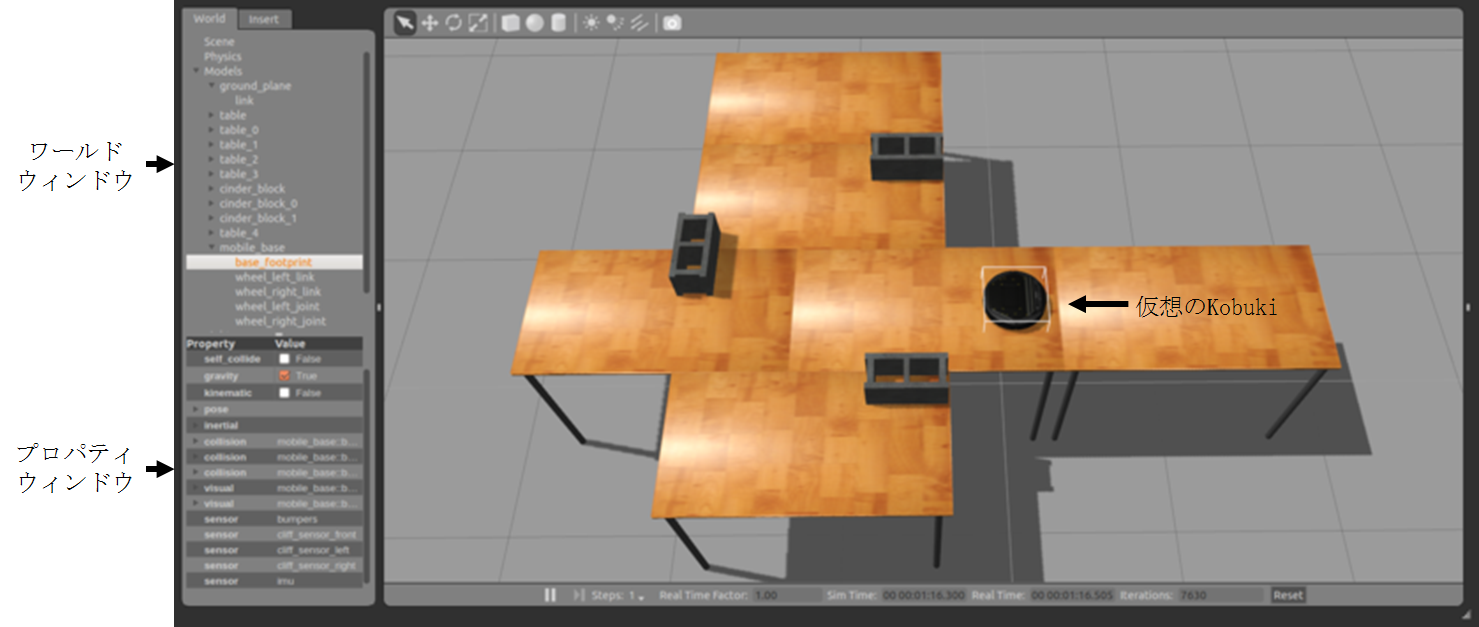
\includegraphics[width=\columnwidth]{pictures/chapter9/pic_09_29.png}
  \caption{kobuki\_playground.launchを実行中の画面}
\end{figure}


本章では、Kobukiパッケージで利用できるシミュレーション環境を2つ紹介した。一つは、ROSの3次元可視化ツールであるRVizを利用する方法であり、もう一つは3次元ロボットシミュレータGazeboを用いる方法である。特にGazeboは動力学計算が可能であり、また外界センサも再現でき、グラフィックス性能も高い。今後はGazeboの利用を推奨したい。

\subsubsection{タートルボットのシミュレーション}

タートルボットは3種類のシミュレーション(stage、stdr、gazebo)をサポートしている。様々なシミュレーション上で仮想ロボットを動作させたい時は、以下の関連Wikiを参考にしてほしい。

http://wiki.ros.org/turtlebot\_stage
http://wiki.ros.org/turtlebot\_stdr
http://wiki.ros.org/turtlebot\_gazebo

% 注1  http://www.willowgarage.com/
% 注2  http://www.osrfoundation.org/
% 注3  http://docs.ros.org/indigo/api/kobuki_msgs/html/msg/SensorState.html
% 注4  http://kobuki.yujinrobot.com/home-en/documentation/howtos/upgrading-firmware/upgrading-firmware-linux/
% 注5  http://files.yujinrobot.com/kobuki/firmware/
% 注6  http://stm32flash.googlecode.com/
% 注7  http://wiki.ros.org/kobuki_auto_docking
% 注8  http://wiki.ros.org/kobuki/Tutorials/Testing%20Automatic%20Docking
% 注9  https://github.com/yujinrobot/kobuki/blob/indigo/kobuki_auto_docking/src/auto_docking_ros.cpp
% 注10 http://wiki.ros.org/kobuki_soft
% 注11 http://gazebosim.org/
% 注12 http://en.wikipedia.org/wiki/Robotics_simulator
% 注13 http://www.darpa.mil/Our_Work/TTO/Programs/DARPA_Robotics_Challenge.aspx
% 注14 http://wiki.ros.org/gazebo_ros_pkgs
% 注15 http://www.ode.org/
% 注16 http://bulletphysics.org/
% 注17 https://simtk.org/home/simbody/
% 注18 http://dartsim.github.io/
% 注19 http://www.ogre3d.org/
% 注20 http://gazebosim.org/api.html
% 注21 http://gazebosim.org/sdf.html
% 注22 https://code.google.com/p/protobuf/
% 注23 http://cloudsim.io/





%-------------------------------------------------------------------------------
